\documentclass[twoside]{book}

% Packages required by doxygen
\usepackage{fixltx2e}
\usepackage{calc}
\usepackage{doxygen}
\usepackage[export]{adjustbox} % also loads graphicx
\usepackage{graphicx}
\usepackage[utf8]{inputenc}
\usepackage{makeidx}
\usepackage{multicol}
\usepackage{multirow}
\PassOptionsToPackage{warn}{textcomp}
\usepackage{textcomp}
\usepackage[nointegrals]{wasysym}
\usepackage[table]{xcolor}

% Font selection
\usepackage[T1]{fontenc}
\usepackage[scaled=.90]{helvet}
\usepackage{courier}
\usepackage{amssymb}
\usepackage{sectsty}
\renewcommand{\familydefault}{\sfdefault}
\allsectionsfont{%
  \fontseries{bc}\selectfont%
  \color{darkgray}%
}
\renewcommand{\DoxyLabelFont}{%
  \fontseries{bc}\selectfont%
  \color{darkgray}%
}
\newcommand{\+}{\discretionary{\mbox{\scriptsize$\hookleftarrow$}}{}{}}

% Page & text layout
\usepackage{geometry}
\geometry{%
  a4paper,%
  top=2.5cm,%
  bottom=2.5cm,%
  left=2.5cm,%
  right=2.5cm%
}
\tolerance=750
\hfuzz=15pt
\hbadness=750
\setlength{\emergencystretch}{15pt}
\setlength{\parindent}{0cm}
\setlength{\parskip}{0.2cm}
\makeatletter
\renewcommand{\paragraph}{%
  \@startsection{paragraph}{4}{0ex}{-1.0ex}{1.0ex}{%
    \normalfont\normalsize\bfseries\SS@parafont%
  }%
}
\renewcommand{\subparagraph}{%
  \@startsection{subparagraph}{5}{0ex}{-1.0ex}{1.0ex}{%
    \normalfont\normalsize\bfseries\SS@subparafont%
  }%
}
\makeatother

% Headers & footers
\usepackage{fancyhdr}
\pagestyle{fancyplain}
\fancyhead[LE]{\fancyplain{}{\bfseries\thepage}}
\fancyhead[CE]{\fancyplain{}{}}
\fancyhead[RE]{\fancyplain{}{\bfseries\leftmark}}
\fancyhead[LO]{\fancyplain{}{\bfseries\rightmark}}
\fancyhead[CO]{\fancyplain{}{}}
\fancyhead[RO]{\fancyplain{}{\bfseries\thepage}}
\fancyfoot[LE]{\fancyplain{}{}}
\fancyfoot[CE]{\fancyplain{}{}}
\fancyfoot[RE]{\fancyplain{}{\bfseries\scriptsize Generated on Wed Sep 30 2015 08\+:46\+:48 for Platform\+Game by Doxygen }}
\fancyfoot[LO]{\fancyplain{}{\bfseries\scriptsize Generated on Wed Sep 30 2015 08\+:46\+:48 for Platform\+Game by Doxygen }}
\fancyfoot[CO]{\fancyplain{}{}}
\fancyfoot[RO]{\fancyplain{}{}}
\renewcommand{\footrulewidth}{0.4pt}
\renewcommand{\chaptermark}[1]{%
  \markboth{#1}{}%
}
\renewcommand{\sectionmark}[1]{%
  \markright{\thesection\ #1}%
}

% Indices & bibliography
\usepackage{natbib}
\usepackage[titles]{tocloft}
\setcounter{tocdepth}{3}
\setcounter{secnumdepth}{5}
\makeindex

% Hyperlinks (required, but should be loaded last)
\usepackage{ifpdf}
\ifpdf
  \usepackage[pdftex,pagebackref=true]{hyperref}
\else
  \usepackage[ps2pdf,pagebackref=true]{hyperref}
\fi
\hypersetup{%
  colorlinks=true,%
  linkcolor=blue,%
  citecolor=blue,%
  unicode%
}

% Custom commands
\newcommand{\clearemptydoublepage}{%
  \newpage{\pagestyle{empty}\cleardoublepage}%
}


%===== C O N T E N T S =====

\begin{document}

% Titlepage & ToC
\hypersetup{pageanchor=false,
             bookmarks=true,
             bookmarksnumbered=true,
             pdfencoding=unicode
            }
\pagenumbering{roman}
\begin{titlepage}
\vspace*{7cm}
\begin{center}%
{\Large Platform\+Game }\\
\vspace*{1cm}
{\large Generated by Doxygen 1.8.10}\\
\vspace*{0.5cm}
{\small Wed Sep 30 2015 08:46:48}\\
\end{center}
\end{titlepage}
\clearemptydoublepage
\tableofcontents
\clearemptydoublepage
\pagenumbering{arabic}
\hypersetup{pageanchor=true}

%--- Begin generated contents ---
\chapter{Hierarchical Index}
\section{Class Hierarchy}
This inheritance list is sorted roughly, but not completely, alphabetically\+:\begin{DoxyCompactList}
\item \contentsline{section}{Abstract\+Entity}{\pageref{class_abstract_entity}}{}
\begin{DoxyCompactList}
\item \contentsline{section}{Graphical\+Entity}{\pageref{class_graphical_entity}}{}
\begin{DoxyCompactList}
\item \contentsline{section}{World\+Entity}{\pageref{class_world_entity}}{}
\begin{DoxyCompactList}
\item \contentsline{section}{Basic\+Platform}{\pageref{class_basic_platform}}{}
\item \contentsline{section}{Basic\+Slope}{\pageref{class_basic_slope}}{}
\item \contentsline{section}{Box\+Boundary}{\pageref{class_box_boundary}}{}
\item \contentsline{section}{Circle}{\pageref{class_circle}}{}
\item \contentsline{section}{Square}{\pageref{class_square}}{}
\item \contentsline{section}{Trail\+Bullet}{\pageref{class_trail_bullet}}{}
\end{DoxyCompactList}
\end{DoxyCompactList}
\item \contentsline{section}{Physical\+Entity}{\pageref{class_physical_entity}}{}
\begin{DoxyCompactList}
\item \contentsline{section}{World\+Entity}{\pageref{class_world_entity}}{}
\end{DoxyCompactList}
\end{DoxyCompactList}
\item \contentsline{section}{Abstract\+Level}{\pageref{class_abstract_level}}{}
\begin{DoxyCompactList}
\item \contentsline{section}{Test\+Level}{\pageref{class_test_level}}{}
\end{DoxyCompactList}
\item b2\+Contact\+Listener\begin{DoxyCompactList}
\item \contentsline{section}{Entity\+Contact\+Listener}{\pageref{class_entity_contact_listener}}{}
\end{DoxyCompactList}
\item Drawable\begin{DoxyCompactList}
\item \contentsline{section}{Graphical\+Element}{\pageref{class_graphical_element}}{}
\end{DoxyCompactList}
\item Transformable\begin{DoxyCompactList}
\item \contentsline{section}{Graphical\+Element}{\pageref{class_graphical_element}}{}
\end{DoxyCompactList}
\end{DoxyCompactList}

\chapter{Class Index}
\section{Class List}
Here are the classes, structs, unions and interfaces with brief descriptions\+:\begin{DoxyCompactList}
\item\contentsline{section}{\hyperlink{class_abstract_entity}{Abstract\+Entity} \\*Contains the \hyperlink{class_abstract_entity}{Abstract\+Entity} class declaration }{\pageref{class_abstract_entity}}{}
\item\contentsline{section}{\hyperlink{class_abstract_level}{Abstract\+Level} \\*Represents a basic linear level, with an end condition }{\pageref{class_abstract_level}}{}
\item\contentsline{section}{\hyperlink{class_basic_platform}{Basic\+Platform} }{\pageref{class_basic_platform}}{}
\item\contentsline{section}{\hyperlink{class_basic_slope}{Basic\+Slope} }{\pageref{class_basic_slope}}{}
\item\contentsline{section}{\hyperlink{class_box_boundary}{Box\+Boundary} }{\pageref{class_box_boundary}}{}
\item\contentsline{section}{\hyperlink{class_circle}{Circle} }{\pageref{class_circle}}{}
\item\contentsline{section}{\hyperlink{class_entity_contact_listener}{Entity\+Contact\+Listener} \\*Contains the \hyperlink{class_entity_contact_listener}{Entity\+Contact\+Listener} class declaration }{\pageref{class_entity_contact_listener}}{}
\item\contentsline{section}{\hyperlink{class_graphical_element}{Graphical\+Element} \\*Contains the \hyperlink{class_graphical_entity}{Graphical\+Entity} and \hyperlink{class_graphical_element}{Graphical\+Element} class declarations }{\pageref{class_graphical_element}}{}
\item\contentsline{section}{\hyperlink{class_graphical_entity}{Graphical\+Entity} \\*Represents a game element that can be displayed }{\pageref{class_graphical_entity}}{}
\item\contentsline{section}{\hyperlink{class_physical_entity}{Physical\+Entity} \\*Contains the \hyperlink{class_physical_entity}{Physical\+Entity} class declaration }{\pageref{class_physical_entity}}{}
\item\contentsline{section}{\hyperlink{class_square}{Square} }{\pageref{class_square}}{}
\item\contentsline{section}{\hyperlink{class_test_level}{Test\+Level} \\*Contains the \hyperlink{class_test_level}{Test\+Level} class declaration }{\pageref{class_test_level}}{}
\item\contentsline{section}{\hyperlink{class_trail_bullet}{Trail\+Bullet} }{\pageref{class_trail_bullet}}{}
\item\contentsline{section}{\hyperlink{class_world_entity}{World\+Entity} \\*Contains the \hyperlink{class_world_entity}{World\+Entity} class declaration }{\pageref{class_world_entity}}{}
\end{DoxyCompactList}

\chapter{File Index}
\section{File List}
Here is a list of all files with brief descriptions\+:\begin{DoxyCompactList}
\item\contentsline{section}{\hyperlink{constants_8hpp}{constants.\+hpp} }{\pageref{constants_8hpp}}{}
\item\contentsline{section}{\hyperlink{main_8cpp}{main.\+cpp} }{\pageref{main_8cpp}}{}
\item\contentsline{section}{\hyperlink{sfml_to_box2_d_8cpp}{sfml\+To\+Box2\+D.\+cpp} }{\pageref{sfml_to_box2_d_8cpp}}{}
\item\contentsline{section}{\hyperlink{sfml_to_box2_d_8hpp}{sfml\+To\+Box2\+D.\+hpp} }{\pageref{sfml_to_box2_d_8hpp}}{}
\item\contentsline{section}{Entity/\hyperlink{_abstract_entity_8hpp}{Abstract\+Entity.\+hpp} }{\pageref{_abstract_entity_8hpp}}{}
\item\contentsline{section}{Entity/\hyperlink{_entity_contact_listener_8cpp}{Entity\+Contact\+Listener.\+cpp} }{\pageref{_entity_contact_listener_8cpp}}{}
\item\contentsline{section}{Entity/\hyperlink{_entity_contact_listener_8hpp}{Entity\+Contact\+Listener.\+hpp} }{\pageref{_entity_contact_listener_8hpp}}{}
\item\contentsline{section}{Entity/\hyperlink{_graphical_entity_8hpp}{Graphical\+Entity.\+hpp} }{\pageref{_graphical_entity_8hpp}}{}
\item\contentsline{section}{Entity/\hyperlink{_physical_entity_8hpp}{Physical\+Entity.\+hpp} }{\pageref{_physical_entity_8hpp}}{}
\item\contentsline{section}{Entity/\hyperlink{_world_entity_8cpp}{World\+Entity.\+cpp} }{\pageref{_world_entity_8cpp}}{}
\item\contentsline{section}{Entity/\hyperlink{_world_entity_8hpp}{World\+Entity.\+hpp} }{\pageref{_world_entity_8hpp}}{}
\item\contentsline{section}{Entity/\+Entities/\hyperlink{_basic_platform_8cpp}{Basic\+Platform.\+cpp} }{\pageref{_basic_platform_8cpp}}{}
\item\contentsline{section}{Entity/\+Entities/\hyperlink{_basic_platform_8hpp}{Basic\+Platform.\+hpp} }{\pageref{_basic_platform_8hpp}}{}
\item\contentsline{section}{Entity/\+Entities/\hyperlink{_basic_slope_8cpp}{Basic\+Slope.\+cpp} }{\pageref{_basic_slope_8cpp}}{}
\item\contentsline{section}{Entity/\+Entities/\hyperlink{_basic_slope_8hpp}{Basic\+Slope.\+hpp} }{\pageref{_basic_slope_8hpp}}{}
\item\contentsline{section}{Entity/\+Entities/\hyperlink{_box_boundary_8cpp}{Box\+Boundary.\+cpp} }{\pageref{_box_boundary_8cpp}}{}
\item\contentsline{section}{Entity/\+Entities/\hyperlink{_box_boundary_8hpp}{Box\+Boundary.\+hpp} }{\pageref{_box_boundary_8hpp}}{}
\item\contentsline{section}{Entity/\+Entities/\hyperlink{_circle_8cpp}{Circle.\+cpp} }{\pageref{_circle_8cpp}}{}
\item\contentsline{section}{Entity/\+Entities/\hyperlink{_circle_8hpp}{Circle.\+hpp} }{\pageref{_circle_8hpp}}{}
\item\contentsline{section}{Entity/\+Entities/\hyperlink{_square_8cpp}{Square.\+cpp} }{\pageref{_square_8cpp}}{}
\item\contentsline{section}{Entity/\+Entities/\hyperlink{_square_8hpp}{Square.\+hpp} }{\pageref{_square_8hpp}}{}
\item\contentsline{section}{Entity/\+Entities/\hyperlink{_trail_bullet_8cpp}{Trail\+Bullet.\+cpp} }{\pageref{_trail_bullet_8cpp}}{}
\item\contentsline{section}{Entity/\+Entities/\hyperlink{_trail_bullet_8hpp}{Trail\+Bullet.\+hpp} }{\pageref{_trail_bullet_8hpp}}{}
\item\contentsline{section}{Level/\hyperlink{_abstract_level_8cpp}{Abstract\+Level.\+cpp} }{\pageref{_abstract_level_8cpp}}{}
\item\contentsline{section}{Level/\hyperlink{_abstract_level_8hpp}{Abstract\+Level.\+hpp} }{\pageref{_abstract_level_8hpp}}{}
\item\contentsline{section}{Level/\+Levels/\hyperlink{_test_level_8cpp}{Test\+Level.\+cpp} }{\pageref{_test_level_8cpp}}{}
\item\contentsline{section}{Level/\+Levels/\hyperlink{_test_level_8hpp}{Test\+Level.\+hpp} }{\pageref{_test_level_8hpp}}{}
\end{DoxyCompactList}

\chapter{Class Documentation}
\hypertarget{class_abstract_entity}{}\section{Abstract\+Entity Class Reference}
\label{class_abstract_entity}\index{Abstract\+Entity@{Abstract\+Entity}}


Contains the \hyperlink{class_abstract_entity}{Abstract\+Entity} class declaration.  




{\ttfamily \#include $<$Abstract\+Entity.\+hpp$>$}

Inheritance diagram for Abstract\+Entity\+:\begin{figure}[H]
\begin{center}
\leavevmode
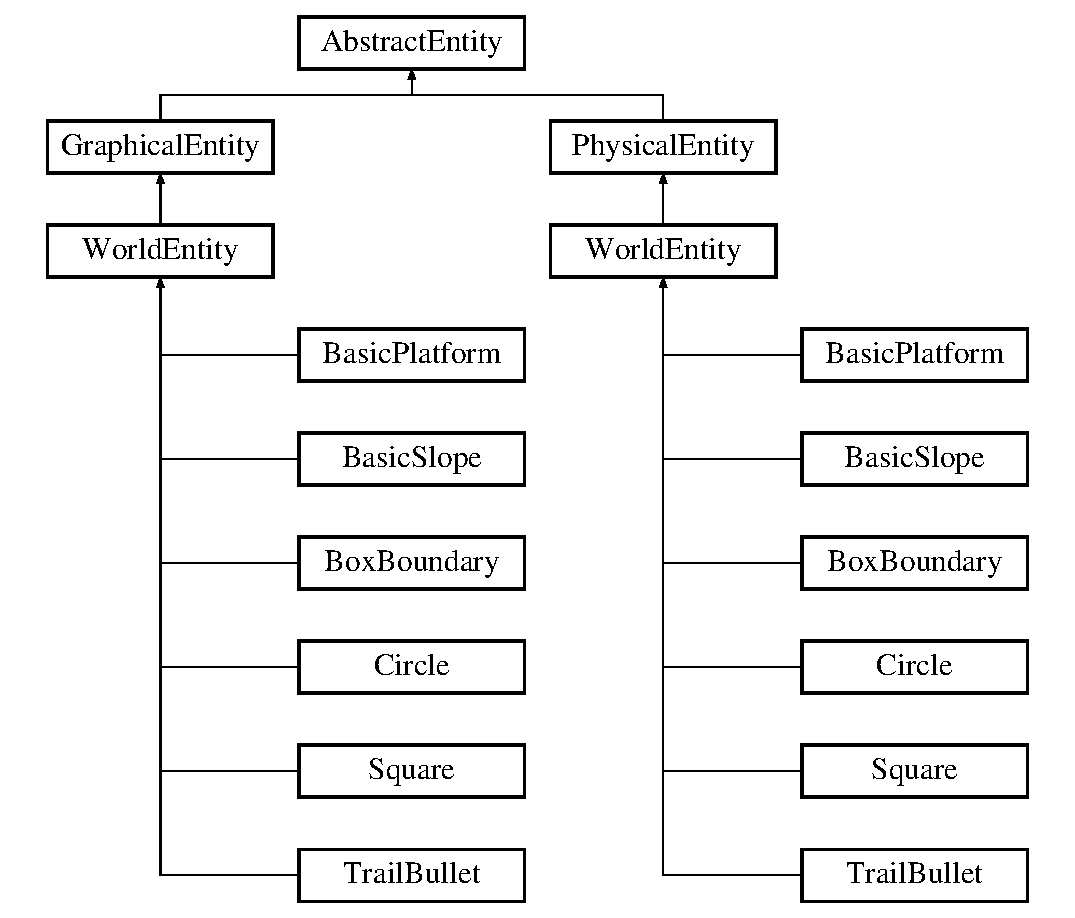
\includegraphics[height=9.000000cm]{class_abstract_entity}
\end{center}
\end{figure}
\subsection*{Public Member Functions}
\begin{DoxyCompactItemize}
\item 
\hyperlink{class_abstract_entity_a4df93a42a764660b849deb5e18efff5e}{Abstract\+Entity} (void)
\begin{DoxyCompactList}\small\item\em Default constructor. \end{DoxyCompactList}\item 
virtual void \hyperlink{class_abstract_entity_ac5602c7978aa4eaff46aa206f06046d7}{tick} (void)=0
\begin{DoxyCompactList}\small\item\em Runs a physical frame of the entity. \end{DoxyCompactList}\item 
virtual \hyperlink{class_abstract_entity_ab5efb435d782e095168ce6199fe2508a}{$\sim$\+Abstract\+Entity} (void)
\begin{DoxyCompactList}\small\item\em Destructor. \end{DoxyCompactList}\item 
bool \hyperlink{class_abstract_entity_a6fa6c7e34a763083ddf813c5f069e400}{is\+Dead} (void) const 
\begin{DoxyCompactList}\small\item\em dead member variable getter. \end{DoxyCompactList}\end{DoxyCompactItemize}
\subsection*{Protected Attributes}
\begin{DoxyCompactItemize}
\item 
bool \hyperlink{class_abstract_entity_acb290d7867b8b032c2535632d270584a}{dead}
\end{DoxyCompactItemize}


\subsection{Detailed Description}
Contains the \hyperlink{class_abstract_entity}{Abstract\+Entity} class declaration. 

\begin{DoxyAuthor}{Author}
Roch Dionnet
\end{DoxyAuthor}
Base class for game entities. 

\subsection{Constructor \& Destructor Documentation}
\hypertarget{class_abstract_entity_a4df93a42a764660b849deb5e18efff5e}{}\index{Abstract\+Entity@{Abstract\+Entity}!Abstract\+Entity@{Abstract\+Entity}}
\index{Abstract\+Entity@{Abstract\+Entity}!Abstract\+Entity@{Abstract\+Entity}}
\subsubsection[{Abstract\+Entity(void)}]{\setlength{\rightskip}{0pt plus 5cm}Abstract\+Entity\+::\+Abstract\+Entity (
\begin{DoxyParamCaption}
\item[{void}]{}
\end{DoxyParamCaption}
)\hspace{0.3cm}{\ttfamily [inline]}}\label{class_abstract_entity_a4df93a42a764660b849deb5e18efff5e}


Default constructor. 

\hypertarget{class_abstract_entity_ab5efb435d782e095168ce6199fe2508a}{}\index{Abstract\+Entity@{Abstract\+Entity}!````~Abstract\+Entity@{$\sim$\+Abstract\+Entity}}
\index{````~Abstract\+Entity@{$\sim$\+Abstract\+Entity}!Abstract\+Entity@{Abstract\+Entity}}
\subsubsection[{$\sim$\+Abstract\+Entity(void)}]{\setlength{\rightskip}{0pt plus 5cm}virtual Abstract\+Entity\+::$\sim$\+Abstract\+Entity (
\begin{DoxyParamCaption}
\item[{void}]{}
\end{DoxyParamCaption}
)\hspace{0.3cm}{\ttfamily [inline]}, {\ttfamily [virtual]}}\label{class_abstract_entity_ab5efb435d782e095168ce6199fe2508a}


Destructor. 



\subsection{Member Function Documentation}
\hypertarget{class_abstract_entity_a6fa6c7e34a763083ddf813c5f069e400}{}\index{Abstract\+Entity@{Abstract\+Entity}!is\+Dead@{is\+Dead}}
\index{is\+Dead@{is\+Dead}!Abstract\+Entity@{Abstract\+Entity}}
\subsubsection[{is\+Dead(void) const }]{\setlength{\rightskip}{0pt plus 5cm}bool Abstract\+Entity\+::is\+Dead (
\begin{DoxyParamCaption}
\item[{void}]{}
\end{DoxyParamCaption}
) const\hspace{0.3cm}{\ttfamily [inline]}}\label{class_abstract_entity_a6fa6c7e34a763083ddf813c5f069e400}


dead member variable getter. 

\begin{DoxyReturn}{Returns}
dead member variable. 
\end{DoxyReturn}
\begin{DoxySeeAlso}{See also}
\hyperlink{class_abstract_entity_acb290d7867b8b032c2535632d270584a}{dead} 
\end{DoxySeeAlso}
\hypertarget{class_abstract_entity_ac5602c7978aa4eaff46aa206f06046d7}{}\index{Abstract\+Entity@{Abstract\+Entity}!tick@{tick}}
\index{tick@{tick}!Abstract\+Entity@{Abstract\+Entity}}
\subsubsection[{tick(void)=0}]{\setlength{\rightskip}{0pt plus 5cm}virtual void Abstract\+Entity\+::tick (
\begin{DoxyParamCaption}
\item[{void}]{}
\end{DoxyParamCaption}
)\hspace{0.3cm}{\ttfamily [pure virtual]}}\label{class_abstract_entity_ac5602c7978aa4eaff46aa206f06046d7}


Runs a physical frame of the entity. 



Implemented in \hyperlink{class_box_boundary_a5f174130498e1cfeb16bd37dfa8bceba}{Box\+Boundary}, \hyperlink{class_square_afb90e037b269f878406d52bee92e7290}{Square}, \hyperlink{class_basic_platform_a4f48429408329c4b0bb8924e410ad44e}{Basic\+Platform}, \hyperlink{class_circle_a352287304dc72826b75108e7333dc6d1}{Circle}, \hyperlink{class_trail_bullet_a3fe11738249bc471194e2eb207730911}{Trail\+Bullet}, and \hyperlink{class_basic_slope_a61be54e264d4dba781efa7d611634aed}{Basic\+Slope}.



\subsection{Member Data Documentation}
\hypertarget{class_abstract_entity_acb290d7867b8b032c2535632d270584a}{}\index{Abstract\+Entity@{Abstract\+Entity}!dead@{dead}}
\index{dead@{dead}!Abstract\+Entity@{Abstract\+Entity}}
\subsubsection[{dead}]{\setlength{\rightskip}{0pt plus 5cm}bool Abstract\+Entity\+::dead\hspace{0.3cm}{\ttfamily [protected]}}\label{class_abstract_entity_acb290d7867b8b032c2535632d270584a}
Tells whether or not the entity is considered as dead. 

The documentation for this class was generated from the following file\+:\begin{DoxyCompactItemize}
\item 
Entity/\hyperlink{_abstract_entity_8hpp}{Abstract\+Entity.\+hpp}\end{DoxyCompactItemize}

\hypertarget{class_abstract_level}{}\section{Abstract\+Level Class Reference}
\label{class_abstract_level}\index{Abstract\+Level@{Abstract\+Level}}


Represents a basic linear level, with an end condition.  




{\ttfamily \#include $<$Abstract\+Level.\+hpp$>$}

Inheritance diagram for Abstract\+Level\+:\begin{figure}[H]
\begin{center}
\leavevmode
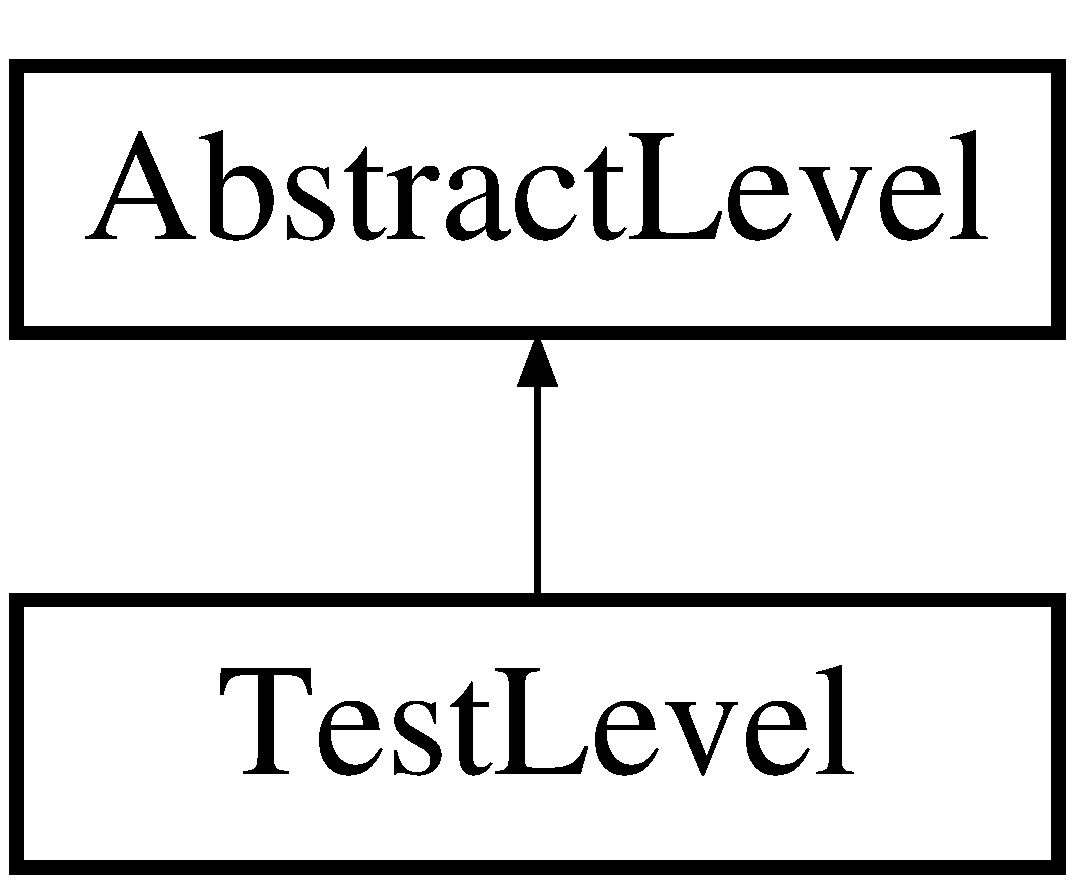
\includegraphics[height=2.000000cm]{class_abstract_level}
\end{center}
\end{figure}
\subsection*{Public Member Functions}
\begin{DoxyCompactItemize}
\item 
\hyperlink{class_abstract_level_a1557b99aa039a0fd5ceb7120306384a1}{Abstract\+Level} (b2\+World \&\hyperlink{class_abstract_level_a566499434bbd056afd9e12b971e8a41e}{world}, sf\+::\+Render\+Window \&\hyperlink{class_abstract_level_a3332e1be17da924be26064ac4e089721}{window})
\begin{DoxyCompactList}\small\item\em Class Constructor. \end{DoxyCompactList}\item 
virtual void \hyperlink{class_abstract_level_aaac7519d2d31d8db995585dec4f5aec0}{initialize} (void)=0
\begin{DoxyCompactList}\small\item\em Initializes the level. Creates the entities and put them in the entity lists, among other things. \end{DoxyCompactList}\item 
virtual void \hyperlink{class_abstract_level_ac50b3069600e90000f2f62dccb522154}{tick} (void)=0
\begin{DoxyCompactList}\small\item\em Game tick. Runs a physical frame of the level. \end{DoxyCompactList}\item 
virtual void \hyperlink{class_abstract_level_aa64f9c76abab71339dc07643472f13ee}{render} (void)
\begin{DoxyCompactList}\small\item\em Render method. Renders the level on screen. \end{DoxyCompactList}\item 
virtual bool \hyperlink{class_abstract_level_a1dbffd34c5ebd93ff833aa6a23047546}{is\+Finished} (void)=0
\begin{DoxyCompactList}\small\item\em Tells whether or not the level is finished. \end{DoxyCompactList}\item 
virtual void \hyperlink{class_abstract_level_aa6b84b35f24206c43bb7cc0af1f9dfb5}{poll\+Event} (sf\+::\+Event e)
\begin{DoxyCompactList}\small\item\em Handles an event caught by the window. \end{DoxyCompactList}\end{DoxyCompactItemize}
\subsection*{Protected Attributes}
\begin{DoxyCompactItemize}
\item 
\hyperlink{_abstract_level_8hpp_a33f40c5b921668406bc9359321c92e00}{Graphical\+Entity\+List} \hyperlink{class_abstract_level_ad08468cc591dab58bbde1dc3ce8ef63d}{graphical\+Entities}
\item 
\hyperlink{_abstract_level_8hpp_a2f8ec60783d4f4d3911b30a32c604d3e}{Physical\+Entity\+List} \hyperlink{class_abstract_level_a3591b89683af2216ef9e958d6e35f863}{physical\+Entities}
\item 
b2\+World \& \hyperlink{class_abstract_level_a566499434bbd056afd9e12b971e8a41e}{world}
\item 
sf\+::\+Render\+Window \& \hyperlink{class_abstract_level_a3332e1be17da924be26064ac4e089721}{window}
\end{DoxyCompactItemize}


\subsection{Detailed Description}
Represents a basic linear level, with an end condition. 

\subsection{Constructor \& Destructor Documentation}
\hypertarget{class_abstract_level_a1557b99aa039a0fd5ceb7120306384a1}{}\index{Abstract\+Level@{Abstract\+Level}!Abstract\+Level@{Abstract\+Level}}
\index{Abstract\+Level@{Abstract\+Level}!Abstract\+Level@{Abstract\+Level}}
\subsubsection[{Abstract\+Level(b2\+World \&world, sf\+::\+Render\+Window \&window)}]{\setlength{\rightskip}{0pt plus 5cm}Abstract\+Level\+::\+Abstract\+Level (
\begin{DoxyParamCaption}
\item[{b2\+World \&}]{world, }
\item[{sf\+::\+Render\+Window \&}]{window}
\end{DoxyParamCaption}
)\hspace{0.3cm}{\ttfamily [inline]}}\label{class_abstract_level_a1557b99aa039a0fd5ceb7120306384a1}


Class Constructor. 


\begin{DoxyParams}{Parameters}
{\em world} & \\
\hline
{\em window} & \\
\hline
\end{DoxyParams}
\begin{DoxySeeAlso}{See also}
\hyperlink{class_abstract_level_a566499434bbd056afd9e12b971e8a41e}{Abstract\+Level\+::world}, \hyperlink{class_abstract_level_a3332e1be17da924be26064ac4e089721}{Abstract\+Level\+::window} 
\end{DoxySeeAlso}


\subsection{Member Function Documentation}
\hypertarget{class_abstract_level_aaac7519d2d31d8db995585dec4f5aec0}{}\index{Abstract\+Level@{Abstract\+Level}!initialize@{initialize}}
\index{initialize@{initialize}!Abstract\+Level@{Abstract\+Level}}
\subsubsection[{initialize(void)=0}]{\setlength{\rightskip}{0pt plus 5cm}virtual void Abstract\+Level\+::initialize (
\begin{DoxyParamCaption}
\item[{void}]{}
\end{DoxyParamCaption}
)\hspace{0.3cm}{\ttfamily [pure virtual]}}\label{class_abstract_level_aaac7519d2d31d8db995585dec4f5aec0}


Initializes the level. Creates the entities and put them in the entity lists, among other things. 



Implemented in \hyperlink{class_test_level_a4be8aacf1a305c58b7670de20d6f4303}{Test\+Level}.

\hypertarget{class_abstract_level_a1dbffd34c5ebd93ff833aa6a23047546}{}\index{Abstract\+Level@{Abstract\+Level}!is\+Finished@{is\+Finished}}
\index{is\+Finished@{is\+Finished}!Abstract\+Level@{Abstract\+Level}}
\subsubsection[{is\+Finished(void)=0}]{\setlength{\rightskip}{0pt plus 5cm}virtual bool Abstract\+Level\+::is\+Finished (
\begin{DoxyParamCaption}
\item[{void}]{}
\end{DoxyParamCaption}
)\hspace{0.3cm}{\ttfamily [pure virtual]}}\label{class_abstract_level_a1dbffd34c5ebd93ff833aa6a23047546}


Tells whether or not the level is finished. 

\begin{DoxyReturn}{Returns}
true if the level\textquotesingle{}s end condition is met, else returns false. 
\end{DoxyReturn}


Implemented in \hyperlink{class_test_level_a2644a0797dc2224ff9088a4c87e71b2b}{Test\+Level}.

\hypertarget{class_abstract_level_aa6b84b35f24206c43bb7cc0af1f9dfb5}{}\index{Abstract\+Level@{Abstract\+Level}!poll\+Event@{poll\+Event}}
\index{poll\+Event@{poll\+Event}!Abstract\+Level@{Abstract\+Level}}
\subsubsection[{poll\+Event(sf\+::\+Event e)}]{\setlength{\rightskip}{0pt plus 5cm}virtual void Abstract\+Level\+::poll\+Event (
\begin{DoxyParamCaption}
\item[{sf\+::\+Event}]{e}
\end{DoxyParamCaption}
)\hspace{0.3cm}{\ttfamily [inline]}, {\ttfamily [virtual]}}\label{class_abstract_level_aa6b84b35f24206c43bb7cc0af1f9dfb5}


Handles an event caught by the window. 


\begin{DoxyParams}{Parameters}
{\em e} & The event to handle. \\
\hline
\end{DoxyParams}


Reimplemented in \hyperlink{class_test_level_a4f16d4600d4b2aeb9299af3417977539}{Test\+Level}.

\hypertarget{class_abstract_level_aa64f9c76abab71339dc07643472f13ee}{}\index{Abstract\+Level@{Abstract\+Level}!render@{render}}
\index{render@{render}!Abstract\+Level@{Abstract\+Level}}
\subsubsection[{render(void)}]{\setlength{\rightskip}{0pt plus 5cm}void Abstract\+Level\+::render (
\begin{DoxyParamCaption}
\item[{void}]{}
\end{DoxyParamCaption}
)\hspace{0.3cm}{\ttfamily [virtual]}}\label{class_abstract_level_aa64f9c76abab71339dc07643472f13ee}


Render method. Renders the level on screen. 



Reimplemented in \hyperlink{class_test_level_a840787cff2a1941a5ce4fafe31433094}{Test\+Level}.

\hypertarget{class_abstract_level_ac50b3069600e90000f2f62dccb522154}{}\index{Abstract\+Level@{Abstract\+Level}!tick@{tick}}
\index{tick@{tick}!Abstract\+Level@{Abstract\+Level}}
\subsubsection[{tick(void)=0}]{\setlength{\rightskip}{0pt plus 5cm}virtual void Abstract\+Level\+::tick (
\begin{DoxyParamCaption}
\item[{void}]{}
\end{DoxyParamCaption}
)\hspace{0.3cm}{\ttfamily [pure virtual]}}\label{class_abstract_level_ac50b3069600e90000f2f62dccb522154}


Game tick. Runs a physical frame of the level. 



Implemented in \hyperlink{class_test_level_a299cc2d19d10678e932bf2df65fe9902}{Test\+Level}.



\subsection{Member Data Documentation}
\hypertarget{class_abstract_level_ad08468cc591dab58bbde1dc3ce8ef63d}{}\index{Abstract\+Level@{Abstract\+Level}!graphical\+Entities@{graphical\+Entities}}
\index{graphical\+Entities@{graphical\+Entities}!Abstract\+Level@{Abstract\+Level}}
\subsubsection[{graphical\+Entities}]{\setlength{\rightskip}{0pt plus 5cm}{\bf Graphical\+Entity\+List} Abstract\+Level\+::graphical\+Entities\hspace{0.3cm}{\ttfamily [protected]}}\label{class_abstract_level_ad08468cc591dab58bbde1dc3ce8ef63d}
Vector of graphical entities. \hypertarget{class_abstract_level_a3591b89683af2216ef9e958d6e35f863}{}\index{Abstract\+Level@{Abstract\+Level}!physical\+Entities@{physical\+Entities}}
\index{physical\+Entities@{physical\+Entities}!Abstract\+Level@{Abstract\+Level}}
\subsubsection[{physical\+Entities}]{\setlength{\rightskip}{0pt plus 5cm}{\bf Physical\+Entity\+List} Abstract\+Level\+::physical\+Entities\hspace{0.3cm}{\ttfamily [protected]}}\label{class_abstract_level_a3591b89683af2216ef9e958d6e35f863}
Vector of physical entities. \hypertarget{class_abstract_level_a3332e1be17da924be26064ac4e089721}{}\index{Abstract\+Level@{Abstract\+Level}!window@{window}}
\index{window@{window}!Abstract\+Level@{Abstract\+Level}}
\subsubsection[{window}]{\setlength{\rightskip}{0pt plus 5cm}sf\+::\+Render\+Window\& Abstract\+Level\+::window\hspace{0.3cm}{\ttfamily [protected]}}\label{class_abstract_level_a3332e1be17da924be26064ac4e089721}
The window that the level is rendered on. \hypertarget{class_abstract_level_a566499434bbd056afd9e12b971e8a41e}{}\index{Abstract\+Level@{Abstract\+Level}!world@{world}}
\index{world@{world}!Abstract\+Level@{Abstract\+Level}}
\subsubsection[{world}]{\setlength{\rightskip}{0pt plus 5cm}b2\+World\& Abstract\+Level\+::world\hspace{0.3cm}{\ttfamily [protected]}}\label{class_abstract_level_a566499434bbd056afd9e12b971e8a41e}
The physical world that the level takes place in. 

The documentation for this class was generated from the following files\+:\begin{DoxyCompactItemize}
\item 
Level/\hyperlink{_abstract_level_8hpp}{Abstract\+Level.\+hpp}\item 
Level/\hyperlink{_abstract_level_8cpp}{Abstract\+Level.\+cpp}\end{DoxyCompactItemize}

\hypertarget{class_basic_platform}{}\section{Basic\+Platform Class Reference}
\label{class_basic_platform}\index{Basic\+Platform@{Basic\+Platform}}


{\ttfamily \#include $<$Basic\+Platform.\+hpp$>$}

Inheritance diagram for Basic\+Platform\+:\begin{figure}[H]
\begin{center}
\leavevmode
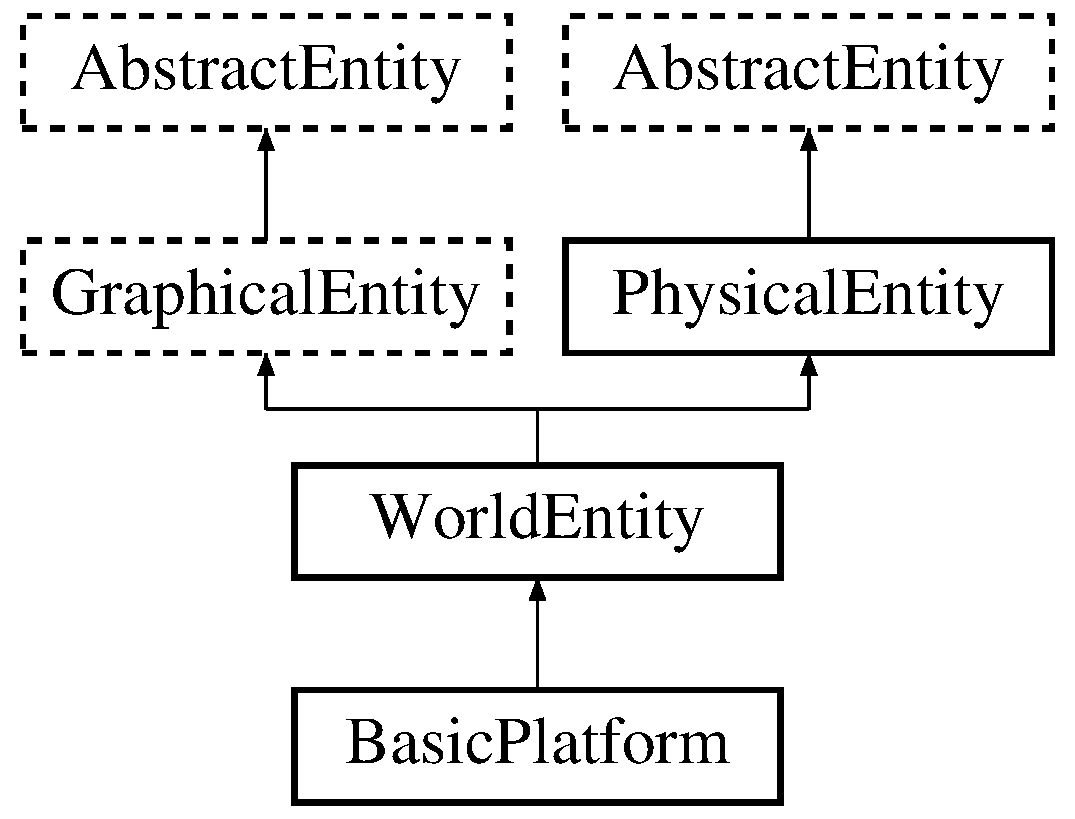
\includegraphics[height=4.000000cm]{class_basic_platform}
\end{center}
\end{figure}
\subsection*{Public Member Functions}
\begin{DoxyCompactItemize}
\item 
\hyperlink{class_basic_platform_aa1c83ff7f1a2f29de3b3e5beb75356ae}{Basic\+Platform} (b2\+World const $\ast$\hyperlink{class_physical_entity_ae6c23c3817c4d7f9a867abed05cd7834}{world}, b2\+Body $\ast$\hyperlink{class_physical_entity_a91a5016393dd890c490b329abd938ec7}{body}, b2\+Vec2 pos, b2\+Vec2 halfsize=\hyperlink{sfml_to_box2_d_8hpp_ae4470ad6d4f3e86df57412ae3dd3dbbc}{graphical\+Vec\+To\+Physical\+Vec}(sf\+::\+Vector2f(256.f, 32.f)))
\item 
virtual void \hyperlink{class_basic_platform_a4f48429408329c4b0bb8924e410ad44e}{tick} (void)
\begin{DoxyCompactList}\small\item\em Runs a physical frame of the entity. \end{DoxyCompactList}\end{DoxyCompactItemize}
\subsection*{Static Public Member Functions}
\begin{DoxyCompactItemize}
\item 
static b2\+Body\+Def \hyperlink{class_basic_platform_ab7dd53f396448d87598661c48696cd9f}{get\+Body\+Def} (void)
\end{DoxyCompactItemize}
\subsection*{Additional Inherited Members}


\subsection{Constructor \& Destructor Documentation}
\hypertarget{class_basic_platform_aa1c83ff7f1a2f29de3b3e5beb75356ae}{}\index{Basic\+Platform@{Basic\+Platform}!Basic\+Platform@{Basic\+Platform}}
\index{Basic\+Platform@{Basic\+Platform}!Basic\+Platform@{Basic\+Platform}}
\subsubsection[{Basic\+Platform(b2\+World const $\ast$world, b2\+Body $\ast$body, b2\+Vec2 pos, b2\+Vec2 halfsize=graphical\+Vec\+To\+Physical\+Vec(sf\+::\+Vector2f(256.\+f, 32.\+f)))}]{\setlength{\rightskip}{0pt plus 5cm}Basic\+Platform\+::\+Basic\+Platform (
\begin{DoxyParamCaption}
\item[{b2\+World const $\ast$}]{world, }
\item[{b2\+Body $\ast$}]{body, }
\item[{b2\+Vec2}]{pos, }
\item[{b2\+Vec2}]{halfsize = {\ttfamily {\bf graphical\+Vec\+To\+Physical\+Vec}(sf\+:\+:Vector2f(256.f,32.f))}}
\end{DoxyParamCaption}
)}\label{class_basic_platform_aa1c83ff7f1a2f29de3b3e5beb75356ae}


\subsection{Member Function Documentation}
\hypertarget{class_basic_platform_ab7dd53f396448d87598661c48696cd9f}{}\index{Basic\+Platform@{Basic\+Platform}!get\+Body\+Def@{get\+Body\+Def}}
\index{get\+Body\+Def@{get\+Body\+Def}!Basic\+Platform@{Basic\+Platform}}
\subsubsection[{get\+Body\+Def(void)}]{\setlength{\rightskip}{0pt plus 5cm}b2\+Body\+Def Basic\+Platform\+::get\+Body\+Def (
\begin{DoxyParamCaption}
\item[{void}]{}
\end{DoxyParamCaption}
)\hspace{0.3cm}{\ttfamily [static]}}\label{class_basic_platform_ab7dd53f396448d87598661c48696cd9f}
\hypertarget{class_basic_platform_a4f48429408329c4b0bb8924e410ad44e}{}\index{Basic\+Platform@{Basic\+Platform}!tick@{tick}}
\index{tick@{tick}!Basic\+Platform@{Basic\+Platform}}
\subsubsection[{tick(void)}]{\setlength{\rightskip}{0pt plus 5cm}virtual void Basic\+Platform\+::tick (
\begin{DoxyParamCaption}
\item[{void}]{}
\end{DoxyParamCaption}
)\hspace{0.3cm}{\ttfamily [inline]}, {\ttfamily [virtual]}}\label{class_basic_platform_a4f48429408329c4b0bb8924e410ad44e}


Runs a physical frame of the entity. 



Implements \hyperlink{class_abstract_entity_ac5602c7978aa4eaff46aa206f06046d7}{Abstract\+Entity}.



The documentation for this class was generated from the following files\+:\begin{DoxyCompactItemize}
\item 
Entity/\+Entities/\hyperlink{_basic_platform_8hpp}{Basic\+Platform.\+hpp}\item 
Entity/\+Entities/\hyperlink{_basic_platform_8cpp}{Basic\+Platform.\+cpp}\end{DoxyCompactItemize}

\hypertarget{class_basic_slope}{}\section{Basic\+Slope Class Reference}
\label{class_basic_slope}\index{Basic\+Slope@{Basic\+Slope}}


{\ttfamily \#include $<$Basic\+Slope.\+hpp$>$}

Inheritance diagram for Basic\+Slope\+:\begin{figure}[H]
\begin{center}
\leavevmode
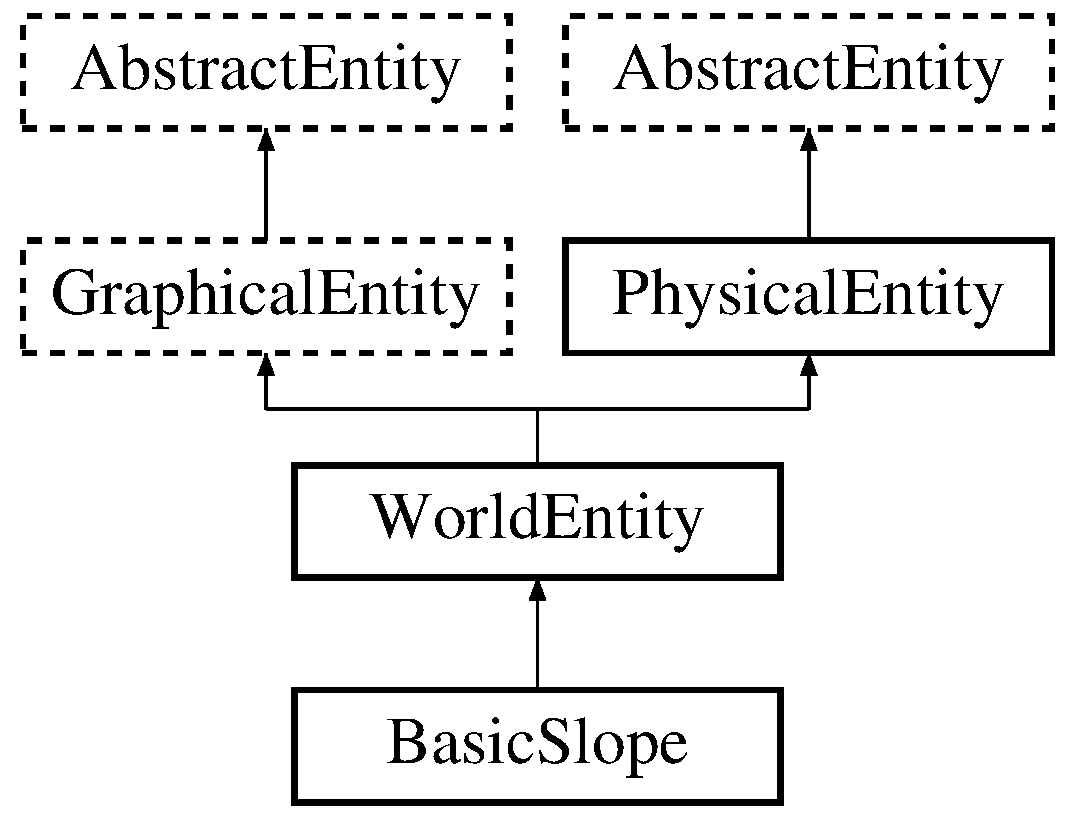
\includegraphics[height=4.000000cm]{class_basic_slope}
\end{center}
\end{figure}
\subsection*{Public Member Functions}
\begin{DoxyCompactItemize}
\item 
\hyperlink{class_basic_slope_afc0a882dcf1f2b03236640c635cfbc46}{Basic\+Slope} (b2\+World const $\ast$\hyperlink{class_physical_entity_ae6c23c3817c4d7f9a867abed05cd7834}{world}, b2\+Body $\ast$\hyperlink{class_physical_entity_a91a5016393dd890c490b329abd938ec7}{body}, b2\+Vec2 pos)
\item 
virtual void \hyperlink{class_basic_slope_a61be54e264d4dba781efa7d611634aed}{tick} (void)
\begin{DoxyCompactList}\small\item\em Runs a physical frame of the entity. \end{DoxyCompactList}\end{DoxyCompactItemize}
\subsection*{Static Public Member Functions}
\begin{DoxyCompactItemize}
\item 
static b2\+Body\+Def \hyperlink{class_basic_slope_a93df874251550b91c9f0ff759c49afdb}{get\+Body\+Def} (void)
\end{DoxyCompactItemize}
\subsection*{Additional Inherited Members}


\subsection{Constructor \& Destructor Documentation}
\hypertarget{class_basic_slope_afc0a882dcf1f2b03236640c635cfbc46}{}\index{Basic\+Slope@{Basic\+Slope}!Basic\+Slope@{Basic\+Slope}}
\index{Basic\+Slope@{Basic\+Slope}!Basic\+Slope@{Basic\+Slope}}
\subsubsection[{Basic\+Slope(b2\+World const $\ast$world, b2\+Body $\ast$body, b2\+Vec2 pos)}]{\setlength{\rightskip}{0pt plus 5cm}Basic\+Slope\+::\+Basic\+Slope (
\begin{DoxyParamCaption}
\item[{b2\+World const $\ast$}]{world, }
\item[{b2\+Body $\ast$}]{body, }
\item[{b2\+Vec2}]{pos}
\end{DoxyParamCaption}
)}\label{class_basic_slope_afc0a882dcf1f2b03236640c635cfbc46}


\subsection{Member Function Documentation}
\hypertarget{class_basic_slope_a93df874251550b91c9f0ff759c49afdb}{}\index{Basic\+Slope@{Basic\+Slope}!get\+Body\+Def@{get\+Body\+Def}}
\index{get\+Body\+Def@{get\+Body\+Def}!Basic\+Slope@{Basic\+Slope}}
\subsubsection[{get\+Body\+Def(void)}]{\setlength{\rightskip}{0pt plus 5cm}b2\+Body\+Def Basic\+Slope\+::get\+Body\+Def (
\begin{DoxyParamCaption}
\item[{void}]{}
\end{DoxyParamCaption}
)\hspace{0.3cm}{\ttfamily [static]}}\label{class_basic_slope_a93df874251550b91c9f0ff759c49afdb}
\hypertarget{class_basic_slope_a61be54e264d4dba781efa7d611634aed}{}\index{Basic\+Slope@{Basic\+Slope}!tick@{tick}}
\index{tick@{tick}!Basic\+Slope@{Basic\+Slope}}
\subsubsection[{tick(void)}]{\setlength{\rightskip}{0pt plus 5cm}virtual void Basic\+Slope\+::tick (
\begin{DoxyParamCaption}
\item[{void}]{}
\end{DoxyParamCaption}
)\hspace{0.3cm}{\ttfamily [inline]}, {\ttfamily [virtual]}}\label{class_basic_slope_a61be54e264d4dba781efa7d611634aed}


Runs a physical frame of the entity. 



Implements \hyperlink{class_abstract_entity_ac5602c7978aa4eaff46aa206f06046d7}{Abstract\+Entity}.



The documentation for this class was generated from the following files\+:\begin{DoxyCompactItemize}
\item 
Entity/\+Entities/\hyperlink{_basic_slope_8hpp}{Basic\+Slope.\+hpp}\item 
Entity/\+Entities/\hyperlink{_basic_slope_8cpp}{Basic\+Slope.\+cpp}\end{DoxyCompactItemize}

\hypertarget{class_box_boundary}{}\section{Box\+Boundary Class Reference}
\label{class_box_boundary}\index{Box\+Boundary@{Box\+Boundary}}


{\ttfamily \#include $<$Box\+Boundary.\+hpp$>$}

Inheritance diagram for Box\+Boundary\+:\begin{figure}[H]
\begin{center}
\leavevmode
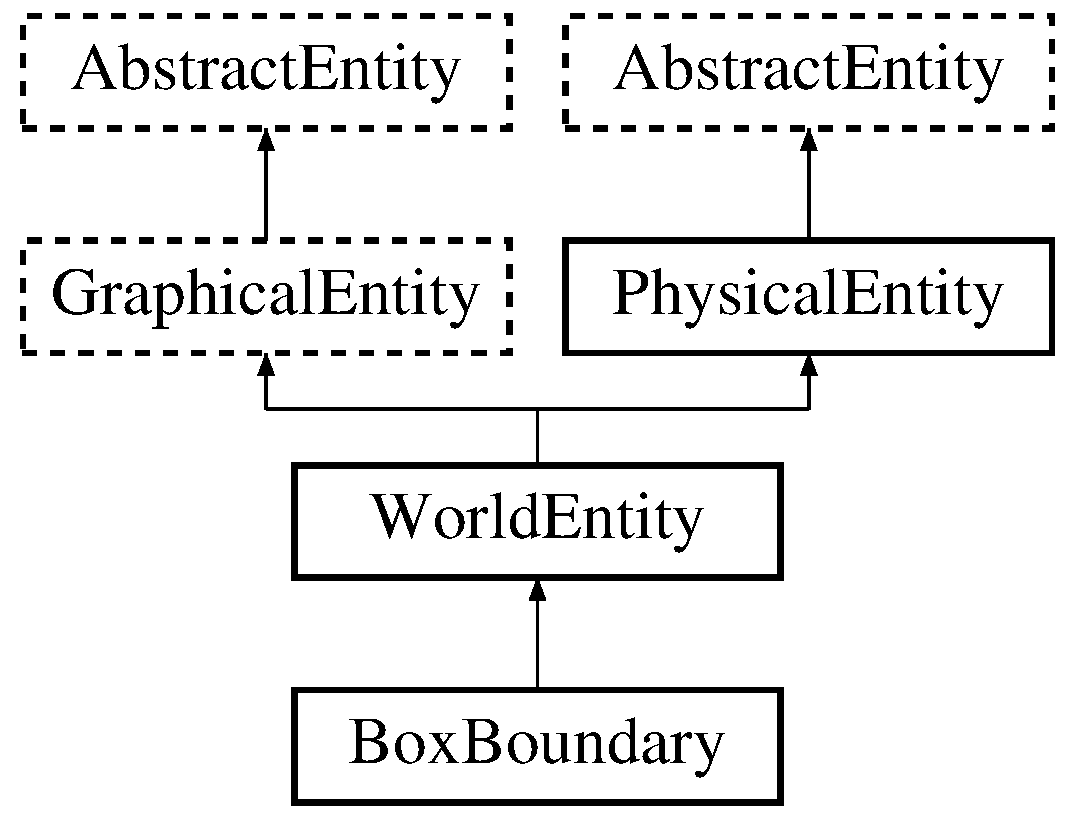
\includegraphics[height=4.000000cm]{class_box_boundary}
\end{center}
\end{figure}
\subsection*{Public Member Functions}
\begin{DoxyCompactItemize}
\item 
\hyperlink{class_box_boundary_aa0fb2fc1d213abc552450e1787c876fd}{Box\+Boundary} (b2\+World const $\ast$\hyperlink{class_physical_entity_ae6c23c3817c4d7f9a867abed05cd7834}{world}, b2\+Body $\ast$\hyperlink{class_physical_entity_a91a5016393dd890c490b329abd938ec7}{body})
\item 
virtual void \hyperlink{class_box_boundary_a5f174130498e1cfeb16bd37dfa8bceba}{tick} (void)
\begin{DoxyCompactList}\small\item\em Runs a physical frame of the entity. \end{DoxyCompactList}\item 
void \hyperlink{class_box_boundary_adedcb98d6617022c19aef0448bf546c5}{set} (b2\+Vec2 pos, b2\+Vec2 size)
\end{DoxyCompactItemize}
\subsection*{Static Public Member Functions}
\begin{DoxyCompactItemize}
\item 
static b2\+Body\+Def \hyperlink{class_box_boundary_a9c23a7955836409c8bc07c3d62cc0637}{get\+Body\+Def} (void)
\end{DoxyCompactItemize}
\subsection*{Additional Inherited Members}


\subsection{Constructor \& Destructor Documentation}
\hypertarget{class_box_boundary_aa0fb2fc1d213abc552450e1787c876fd}{}\index{Box\+Boundary@{Box\+Boundary}!Box\+Boundary@{Box\+Boundary}}
\index{Box\+Boundary@{Box\+Boundary}!Box\+Boundary@{Box\+Boundary}}
\subsubsection[{Box\+Boundary(b2\+World const $\ast$world, b2\+Body $\ast$body)}]{\setlength{\rightskip}{0pt plus 5cm}Box\+Boundary\+::\+Box\+Boundary (
\begin{DoxyParamCaption}
\item[{b2\+World const $\ast$}]{world, }
\item[{b2\+Body $\ast$}]{body}
\end{DoxyParamCaption}
)\hspace{0.3cm}{\ttfamily [inline]}}\label{class_box_boundary_aa0fb2fc1d213abc552450e1787c876fd}


\subsection{Member Function Documentation}
\hypertarget{class_box_boundary_a9c23a7955836409c8bc07c3d62cc0637}{}\index{Box\+Boundary@{Box\+Boundary}!get\+Body\+Def@{get\+Body\+Def}}
\index{get\+Body\+Def@{get\+Body\+Def}!Box\+Boundary@{Box\+Boundary}}
\subsubsection[{get\+Body\+Def(void)}]{\setlength{\rightskip}{0pt plus 5cm}b2\+Body\+Def Box\+Boundary\+::get\+Body\+Def (
\begin{DoxyParamCaption}
\item[{void}]{}
\end{DoxyParamCaption}
)\hspace{0.3cm}{\ttfamily [static]}}\label{class_box_boundary_a9c23a7955836409c8bc07c3d62cc0637}
\hypertarget{class_box_boundary_adedcb98d6617022c19aef0448bf546c5}{}\index{Box\+Boundary@{Box\+Boundary}!set@{set}}
\index{set@{set}!Box\+Boundary@{Box\+Boundary}}
\subsubsection[{set(b2\+Vec2 pos, b2\+Vec2 size)}]{\setlength{\rightskip}{0pt plus 5cm}void Box\+Boundary\+::set (
\begin{DoxyParamCaption}
\item[{b2\+Vec2}]{pos, }
\item[{b2\+Vec2}]{size}
\end{DoxyParamCaption}
)}\label{class_box_boundary_adedcb98d6617022c19aef0448bf546c5}
\hypertarget{class_box_boundary_a5f174130498e1cfeb16bd37dfa8bceba}{}\index{Box\+Boundary@{Box\+Boundary}!tick@{tick}}
\index{tick@{tick}!Box\+Boundary@{Box\+Boundary}}
\subsubsection[{tick(void)}]{\setlength{\rightskip}{0pt plus 5cm}virtual void Box\+Boundary\+::tick (
\begin{DoxyParamCaption}
\item[{void}]{}
\end{DoxyParamCaption}
)\hspace{0.3cm}{\ttfamily [inline]}, {\ttfamily [virtual]}}\label{class_box_boundary_a5f174130498e1cfeb16bd37dfa8bceba}


Runs a physical frame of the entity. 



Implements \hyperlink{class_abstract_entity_ac5602c7978aa4eaff46aa206f06046d7}{Abstract\+Entity}.



The documentation for this class was generated from the following files\+:\begin{DoxyCompactItemize}
\item 
Entity/\+Entities/\hyperlink{_box_boundary_8hpp}{Box\+Boundary.\+hpp}\item 
Entity/\+Entities/\hyperlink{_box_boundary_8cpp}{Box\+Boundary.\+cpp}\end{DoxyCompactItemize}

\hypertarget{class_circle}{}\section{Circle Class Reference}
\label{class_circle}\index{Circle@{Circle}}


{\ttfamily \#include $<$Circle.\+hpp$>$}

Inheritance diagram for Circle\+:\begin{figure}[H]
\begin{center}
\leavevmode
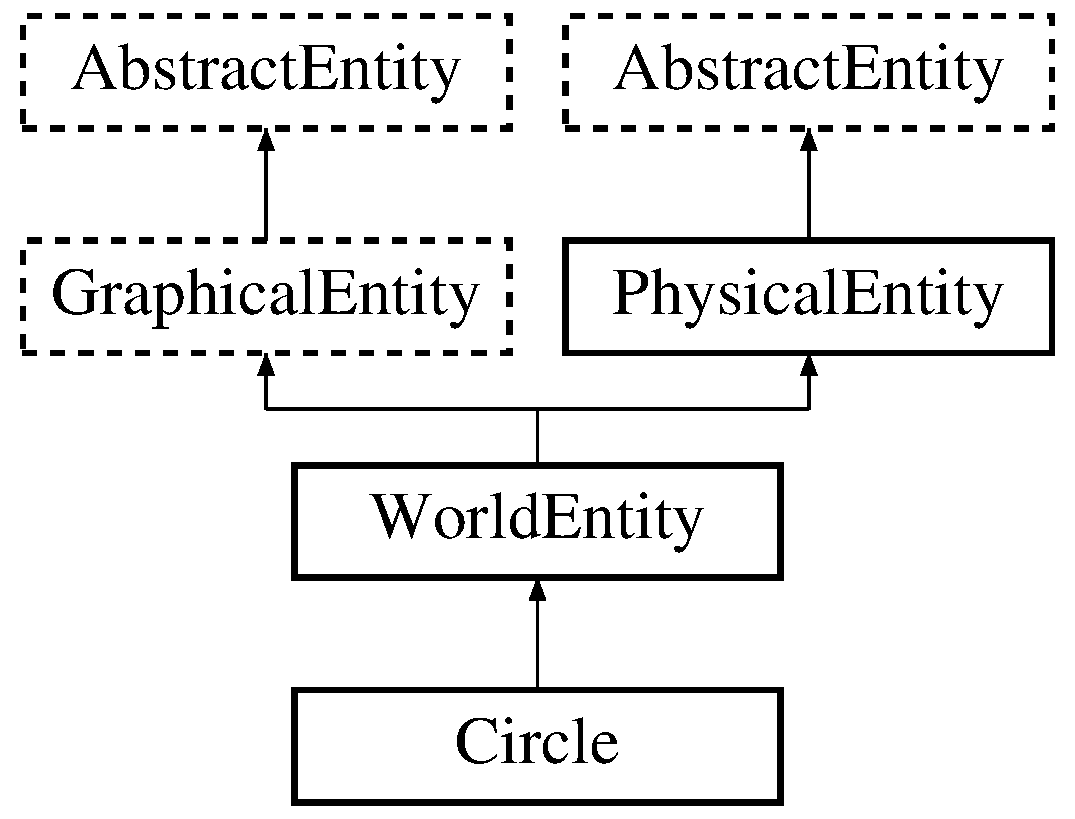
\includegraphics[height=4.000000cm]{class_circle}
\end{center}
\end{figure}
\subsection*{Public Member Functions}
\begin{DoxyCompactItemize}
\item 
\hyperlink{class_circle_a7e86a4697d23fba03002e859070536c5}{Circle} (b2\+World const $\ast$\hyperlink{class_physical_entity_ae6c23c3817c4d7f9a867abed05cd7834}{world}, b2\+Body $\ast$\hyperlink{class_physical_entity_a91a5016393dd890c490b329abd938ec7}{body})
\item 
virtual void \hyperlink{class_circle_a352287304dc72826b75108e7333dc6d1}{tick} (void)
\begin{DoxyCompactList}\small\item\em Runs a physical frame of the entity. \end{DoxyCompactList}\end{DoxyCompactItemize}
\subsection*{Static Public Member Functions}
\begin{DoxyCompactItemize}
\item 
static b2\+Body\+Def \hyperlink{class_circle_aa3f08fbafb89c33743b16136c30a3e50}{get\+Body\+Def} (void)
\end{DoxyCompactItemize}
\subsection*{Additional Inherited Members}


\subsection{Constructor \& Destructor Documentation}
\hypertarget{class_circle_a7e86a4697d23fba03002e859070536c5}{}\index{Circle@{Circle}!Circle@{Circle}}
\index{Circle@{Circle}!Circle@{Circle}}
\subsubsection[{Circle(b2\+World const $\ast$world, b2\+Body $\ast$body)}]{\setlength{\rightskip}{0pt plus 5cm}Circle\+::\+Circle (
\begin{DoxyParamCaption}
\item[{b2\+World const $\ast$}]{world, }
\item[{b2\+Body $\ast$}]{body}
\end{DoxyParamCaption}
)}\label{class_circle_a7e86a4697d23fba03002e859070536c5}


\subsection{Member Function Documentation}
\hypertarget{class_circle_aa3f08fbafb89c33743b16136c30a3e50}{}\index{Circle@{Circle}!get\+Body\+Def@{get\+Body\+Def}}
\index{get\+Body\+Def@{get\+Body\+Def}!Circle@{Circle}}
\subsubsection[{get\+Body\+Def(void)}]{\setlength{\rightskip}{0pt plus 5cm}b2\+Body\+Def Circle\+::get\+Body\+Def (
\begin{DoxyParamCaption}
\item[{void}]{}
\end{DoxyParamCaption}
)\hspace{0.3cm}{\ttfamily [static]}}\label{class_circle_aa3f08fbafb89c33743b16136c30a3e50}
\hypertarget{class_circle_a352287304dc72826b75108e7333dc6d1}{}\index{Circle@{Circle}!tick@{tick}}
\index{tick@{tick}!Circle@{Circle}}
\subsubsection[{tick(void)}]{\setlength{\rightskip}{0pt plus 5cm}void Circle\+::tick (
\begin{DoxyParamCaption}
\item[{void}]{}
\end{DoxyParamCaption}
)\hspace{0.3cm}{\ttfamily [virtual]}}\label{class_circle_a352287304dc72826b75108e7333dc6d1}


Runs a physical frame of the entity. 



Implements \hyperlink{class_abstract_entity_ac5602c7978aa4eaff46aa206f06046d7}{Abstract\+Entity}.



The documentation for this class was generated from the following files\+:\begin{DoxyCompactItemize}
\item 
Entity/\+Entities/\hyperlink{_circle_8hpp}{Circle.\+hpp}\item 
Entity/\+Entities/\hyperlink{_circle_8cpp}{Circle.\+cpp}\end{DoxyCompactItemize}

\hypertarget{class_entity_contact_listener}{}\section{Entity\+Contact\+Listener Class Reference}
\label{class_entity_contact_listener}\index{Entity\+Contact\+Listener@{Entity\+Contact\+Listener}}


Contains the \hyperlink{class_entity_contact_listener}{Entity\+Contact\+Listener} class declaration.  




{\ttfamily \#include $<$Entity\+Contact\+Listener.\+hpp$>$}

Inheritance diagram for Entity\+Contact\+Listener\+:\begin{figure}[H]
\begin{center}
\leavevmode
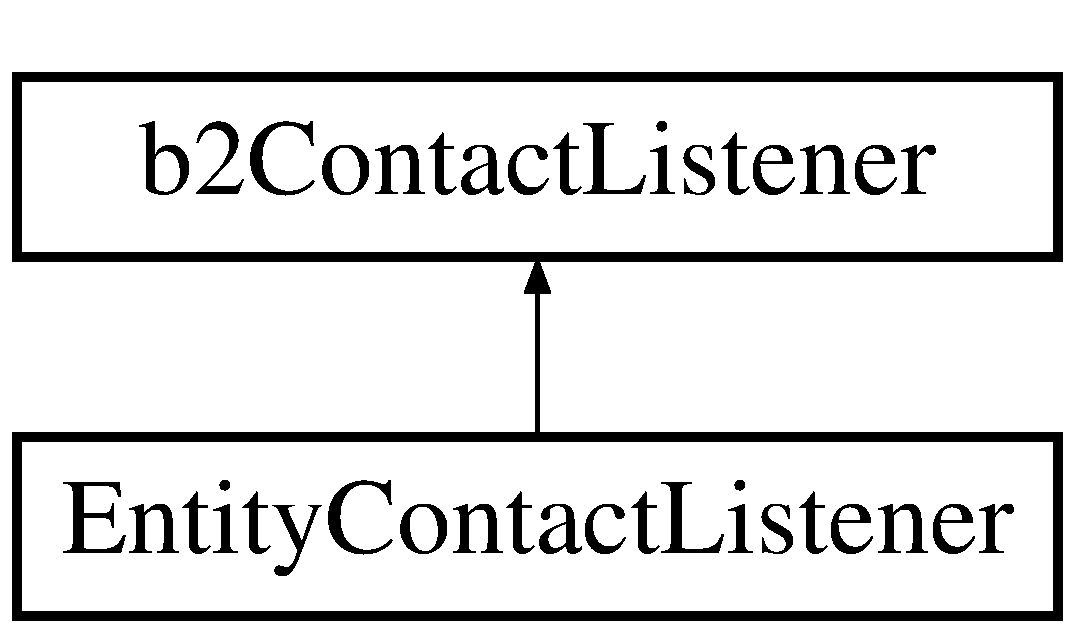
\includegraphics[height=2.000000cm]{class_entity_contact_listener}
\end{center}
\end{figure}
\subsection*{Public Member Functions}
\begin{DoxyCompactItemize}
\item 
void \hyperlink{class_entity_contact_listener_a39de8f983393da191320b0b3c0b85479}{Begin\+Contact} (b2\+Contact $\ast$contact)
\begin{DoxyCompactList}\small\item\em Delegates begin\+Contact management to the entity it is related to. \end{DoxyCompactList}\item 
void \hyperlink{class_entity_contact_listener_a5249dbe70cfb30d2e3aa629424bb66ab}{End\+Contact} (b2\+Contact $\ast$contact)
\begin{DoxyCompactList}\small\item\em Delegates end\+Contact management to the entity it is related to. \end{DoxyCompactList}\end{DoxyCompactItemize}


\subsection{Detailed Description}
Contains the \hyperlink{class_entity_contact_listener}{Entity\+Contact\+Listener} class declaration. 

\begin{DoxyAuthor}{Author}
Roch Dionnet
\end{DoxyAuthor}
A contact listener for entities. 

\subsection{Member Function Documentation}
\hypertarget{class_entity_contact_listener_a39de8f983393da191320b0b3c0b85479}{}\index{Entity\+Contact\+Listener@{Entity\+Contact\+Listener}!Begin\+Contact@{Begin\+Contact}}
\index{Begin\+Contact@{Begin\+Contact}!Entity\+Contact\+Listener@{Entity\+Contact\+Listener}}
\subsubsection[{Begin\+Contact(b2\+Contact $\ast$contact)}]{\setlength{\rightskip}{0pt plus 5cm}void Entity\+Contact\+Listener\+::\+Begin\+Contact (
\begin{DoxyParamCaption}
\item[{b2\+Contact $\ast$}]{contact}
\end{DoxyParamCaption}
)}\label{class_entity_contact_listener_a39de8f983393da191320b0b3c0b85479}


Delegates begin\+Contact management to the entity it is related to. 


\begin{DoxyParams}{Parameters}
{\em contact} & The contact information. \\
\hline
\end{DoxyParams}
\hypertarget{class_entity_contact_listener_a5249dbe70cfb30d2e3aa629424bb66ab}{}\index{Entity\+Contact\+Listener@{Entity\+Contact\+Listener}!End\+Contact@{End\+Contact}}
\index{End\+Contact@{End\+Contact}!Entity\+Contact\+Listener@{Entity\+Contact\+Listener}}
\subsubsection[{End\+Contact(b2\+Contact $\ast$contact)}]{\setlength{\rightskip}{0pt plus 5cm}void Entity\+Contact\+Listener\+::\+End\+Contact (
\begin{DoxyParamCaption}
\item[{b2\+Contact $\ast$}]{contact}
\end{DoxyParamCaption}
)}\label{class_entity_contact_listener_a5249dbe70cfb30d2e3aa629424bb66ab}


Delegates end\+Contact management to the entity it is related to. 


\begin{DoxyParams}{Parameters}
{\em contact} & The contact information. \\
\hline
\end{DoxyParams}


The documentation for this class was generated from the following files\+:\begin{DoxyCompactItemize}
\item 
Entity/\hyperlink{_entity_contact_listener_8hpp}{Entity\+Contact\+Listener.\+hpp}\item 
Entity/\hyperlink{_entity_contact_listener_8cpp}{Entity\+Contact\+Listener.\+cpp}\end{DoxyCompactItemize}

\hypertarget{class_graphical_element}{}\section{Graphical\+Element Class Reference}
\label{class_graphical_element}\index{Graphical\+Element@{Graphical\+Element}}


Contains the \hyperlink{class_graphical_entity}{Graphical\+Entity} and \hyperlink{class_graphical_element}{Graphical\+Element} class declarations.  




{\ttfamily \#include $<$Graphical\+Entity.\+hpp$>$}

Inheritance diagram for Graphical\+Element\+:\begin{figure}[H]
\begin{center}
\leavevmode
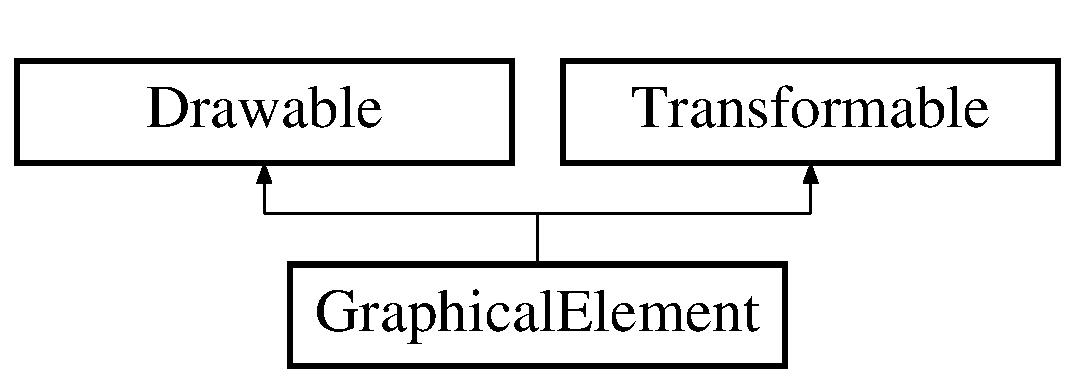
\includegraphics[height=2.000000cm]{class_graphical_element}
\end{center}
\end{figure}


\subsection{Detailed Description}
Contains the \hyperlink{class_graphical_entity}{Graphical\+Entity} and \hyperlink{class_graphical_element}{Graphical\+Element} class declarations. 

\begin{DoxyAuthor}{Author}
Roch Dionnet
\end{DoxyAuthor}
This class is used to represent an element that is both transformable and drawable. With polymorphism, it can be used as an S\+F\+M\+L Sprite or an S\+F\+M\+L Shape. 

The documentation for this class was generated from the following file\+:\begin{DoxyCompactItemize}
\item 
Entity/\hyperlink{_graphical_entity_8hpp}{Graphical\+Entity.\+hpp}\end{DoxyCompactItemize}

\hypertarget{class_graphical_entity}{}\section{Graphical\+Entity Class Reference}
\label{class_graphical_entity}\index{Graphical\+Entity@{Graphical\+Entity}}


Represents a game element that can be displayed.  




{\ttfamily \#include $<$Graphical\+Entity.\+hpp$>$}

Inheritance diagram for Graphical\+Entity\+:\begin{figure}[H]
\begin{center}
\leavevmode
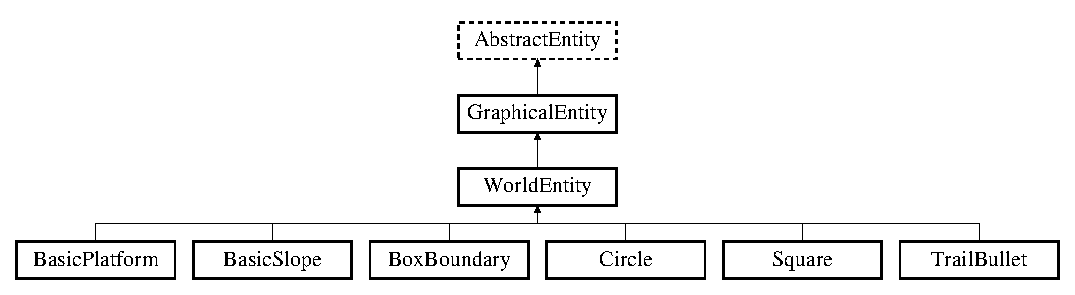
\includegraphics[height=3.522013cm]{class_graphical_entity}
\end{center}
\end{figure}
\subsection*{Public Member Functions}
\begin{DoxyCompactItemize}
\item 
\hyperlink{class_graphical_entity_af5d385d6973e4547e11a26123a747c9d}{Graphical\+Entity} (void)
\begin{DoxyCompactList}\small\item\em Default constructor. \end{DoxyCompactList}\item 
virtual \hyperlink{class_graphical_entity_a1004dcb764464cd2112b9e2ae155189d}{$\sim$\+Graphical\+Entity} (void)
\begin{DoxyCompactList}\small\item\em Virtual destructor. \end{DoxyCompactList}\item 
\hyperlink{class_graphical_element}{Graphical\+Element} const $\ast$ \hyperlink{class_graphical_entity_ac83fdd85a8d7ef87d65534bf0644da24}{get\+Graphical\+Element} (void) const 
\begin{DoxyCompactList}\small\item\em graphical\+Element class variable getter. \end{DoxyCompactList}\end{DoxyCompactItemize}
\subsection*{Protected Attributes}
\begin{DoxyCompactItemize}
\item 
\hyperlink{class_graphical_element}{Graphical\+Element} $\ast$ \hyperlink{class_graphical_entity_a02c6206c0101ab3f8262ec8f0622e883}{graphical\+Element}
\end{DoxyCompactItemize}


\subsection{Detailed Description}
Represents a game element that can be displayed. 

\subsection{Constructor \& Destructor Documentation}
\hypertarget{class_graphical_entity_af5d385d6973e4547e11a26123a747c9d}{}\index{Graphical\+Entity@{Graphical\+Entity}!Graphical\+Entity@{Graphical\+Entity}}
\index{Graphical\+Entity@{Graphical\+Entity}!Graphical\+Entity@{Graphical\+Entity}}
\subsubsection[{Graphical\+Entity(void)}]{\setlength{\rightskip}{0pt plus 5cm}Graphical\+Entity\+::\+Graphical\+Entity (
\begin{DoxyParamCaption}
\item[{void}]{}
\end{DoxyParamCaption}
)\hspace{0.3cm}{\ttfamily [inline]}}\label{class_graphical_entity_af5d385d6973e4547e11a26123a747c9d}


Default constructor. 

\hypertarget{class_graphical_entity_a1004dcb764464cd2112b9e2ae155189d}{}\index{Graphical\+Entity@{Graphical\+Entity}!````~Graphical\+Entity@{$\sim$\+Graphical\+Entity}}
\index{````~Graphical\+Entity@{$\sim$\+Graphical\+Entity}!Graphical\+Entity@{Graphical\+Entity}}
\subsubsection[{$\sim$\+Graphical\+Entity(void)}]{\setlength{\rightskip}{0pt plus 5cm}virtual Graphical\+Entity\+::$\sim$\+Graphical\+Entity (
\begin{DoxyParamCaption}
\item[{void}]{}
\end{DoxyParamCaption}
)\hspace{0.3cm}{\ttfamily [inline]}, {\ttfamily [virtual]}}\label{class_graphical_entity_a1004dcb764464cd2112b9e2ae155189d}


Virtual destructor. 



\subsection{Member Function Documentation}
\hypertarget{class_graphical_entity_ac83fdd85a8d7ef87d65534bf0644da24}{}\index{Graphical\+Entity@{Graphical\+Entity}!get\+Graphical\+Element@{get\+Graphical\+Element}}
\index{get\+Graphical\+Element@{get\+Graphical\+Element}!Graphical\+Entity@{Graphical\+Entity}}
\subsubsection[{get\+Graphical\+Element(void) const }]{\setlength{\rightskip}{0pt plus 5cm}{\bf Graphical\+Element} const$\ast$ Graphical\+Entity\+::get\+Graphical\+Element (
\begin{DoxyParamCaption}
\item[{void}]{}
\end{DoxyParamCaption}
) const\hspace{0.3cm}{\ttfamily [inline]}}\label{class_graphical_entity_ac83fdd85a8d7ef87d65534bf0644da24}


graphical\+Element class variable getter. 

\begin{DoxyReturn}{Returns}
the graphical\+Element class variable. 
\end{DoxyReturn}


\subsection{Member Data Documentation}
\hypertarget{class_graphical_entity_a02c6206c0101ab3f8262ec8f0622e883}{}\index{Graphical\+Entity@{Graphical\+Entity}!graphical\+Element@{graphical\+Element}}
\index{graphical\+Element@{graphical\+Element}!Graphical\+Entity@{Graphical\+Entity}}
\subsubsection[{graphical\+Element}]{\setlength{\rightskip}{0pt plus 5cm}{\bf Graphical\+Element}$\ast$ Graphical\+Entity\+::graphical\+Element\hspace{0.3cm}{\ttfamily [protected]}}\label{class_graphical_entity_a02c6206c0101ab3f8262ec8f0622e883}
A pointer on the graphical\+Element that can be displayed 

The documentation for this class was generated from the following file\+:\begin{DoxyCompactItemize}
\item 
Entity/\hyperlink{_graphical_entity_8hpp}{Graphical\+Entity.\+hpp}\end{DoxyCompactItemize}

\hypertarget{class_physical_entity}{}\section{Physical\+Entity Class Reference}
\label{class_physical_entity}\index{Physical\+Entity@{Physical\+Entity}}


Contains the \hyperlink{class_physical_entity}{Physical\+Entity} class declaration.  




{\ttfamily \#include $<$Physical\+Entity.\+hpp$>$}

Inheritance diagram for Physical\+Entity\+:\begin{figure}[H]
\begin{center}
\leavevmode
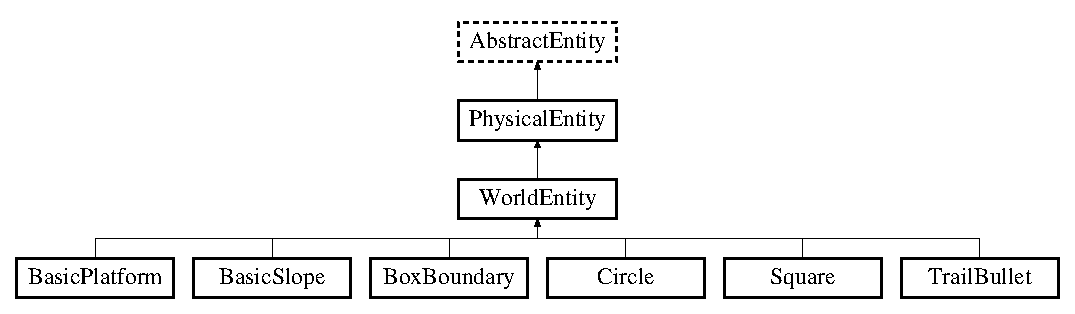
\includegraphics[height=3.771044cm]{class_physical_entity}
\end{center}
\end{figure}
\subsection*{Public Member Functions}
\begin{DoxyCompactItemize}
\item 
\hyperlink{class_physical_entity_a7e10473f085a0032f0d9c6b17641c777}{Physical\+Entity} (b2\+World const $\ast$\hyperlink{class_physical_entity_ae6c23c3817c4d7f9a867abed05cd7834}{world}, b2\+Body $\ast$\hyperlink{class_physical_entity_a91a5016393dd890c490b329abd938ec7}{body})
\begin{DoxyCompactList}\small\item\em Constructor. \end{DoxyCompactList}\item 
b2\+Body $\ast$ \hyperlink{class_physical_entity_aaf3369e0c6147c0280a3abca28a75e96}{get\+Body} (void) const 
\begin{DoxyCompactList}\small\item\em body member variable getter. \end{DoxyCompactList}\item 
virtual void \hyperlink{class_physical_entity_a61e9f273e51f5855ca0bf7bb842c738d}{on\+Begin\+Contact} (b2\+Contact $\ast$contact)
\begin{DoxyCompactList}\small\item\em Contains what the entity should do when a contact begins. \end{DoxyCompactList}\item 
virtual void \hyperlink{class_physical_entity_ae2a98ad512ba0169dcca7bb5b4223306}{on\+End\+Contact} (b2\+Contact $\ast$contact)
\begin{DoxyCompactList}\small\item\em Contains what the entity shoukd do when a contact ends. \end{DoxyCompactList}\end{DoxyCompactItemize}
\subsection*{Protected Attributes}
\begin{DoxyCompactItemize}
\item 
b2\+Body $\ast$ \hyperlink{class_physical_entity_a91a5016393dd890c490b329abd938ec7}{body}
\item 
b2\+World const $\ast$ \hyperlink{class_physical_entity_ae6c23c3817c4d7f9a867abed05cd7834}{world}
\end{DoxyCompactItemize}


\subsection{Detailed Description}
Contains the \hyperlink{class_physical_entity}{Physical\+Entity} class declaration. 

\begin{DoxyAuthor}{Author}
Roch Dionnet
\end{DoxyAuthor}
Represents a game element, physics-\/wise. 

\subsection{Constructor \& Destructor Documentation}
\hypertarget{class_physical_entity_a7e10473f085a0032f0d9c6b17641c777}{}\index{Physical\+Entity@{Physical\+Entity}!Physical\+Entity@{Physical\+Entity}}
\index{Physical\+Entity@{Physical\+Entity}!Physical\+Entity@{Physical\+Entity}}
\subsubsection[{Physical\+Entity(b2\+World const $\ast$world, b2\+Body $\ast$body)}]{\setlength{\rightskip}{0pt plus 5cm}Physical\+Entity\+::\+Physical\+Entity (
\begin{DoxyParamCaption}
\item[{b2\+World const $\ast$}]{world, }
\item[{b2\+Body $\ast$}]{body}
\end{DoxyParamCaption}
)\hspace{0.3cm}{\ttfamily [inline]}}\label{class_physical_entity_a7e10473f085a0032f0d9c6b17641c777}


Constructor. 


\begin{DoxyParams}{Parameters}
{\em world} & \\
\hline
{\em body} & \\
\hline
\end{DoxyParams}
\begin{DoxySeeAlso}{See also}
\hyperlink{class_physical_entity_ae6c23c3817c4d7f9a867abed05cd7834}{Physical\+Entity\+::world}, \hyperlink{class_physical_entity_a91a5016393dd890c490b329abd938ec7}{Physical\+Entity\+::body} 
\end{DoxySeeAlso}


\subsection{Member Function Documentation}
\hypertarget{class_physical_entity_aaf3369e0c6147c0280a3abca28a75e96}{}\index{Physical\+Entity@{Physical\+Entity}!get\+Body@{get\+Body}}
\index{get\+Body@{get\+Body}!Physical\+Entity@{Physical\+Entity}}
\subsubsection[{get\+Body(void) const }]{\setlength{\rightskip}{0pt plus 5cm}b2\+Body$\ast$ Physical\+Entity\+::get\+Body (
\begin{DoxyParamCaption}
\item[{void}]{}
\end{DoxyParamCaption}
) const\hspace{0.3cm}{\ttfamily [inline]}}\label{class_physical_entity_aaf3369e0c6147c0280a3abca28a75e96}


body member variable getter. 

\begin{DoxyReturn}{Returns}
The body member variable. 
\end{DoxyReturn}
\hypertarget{class_physical_entity_a61e9f273e51f5855ca0bf7bb842c738d}{}\index{Physical\+Entity@{Physical\+Entity}!on\+Begin\+Contact@{on\+Begin\+Contact}}
\index{on\+Begin\+Contact@{on\+Begin\+Contact}!Physical\+Entity@{Physical\+Entity}}
\subsubsection[{on\+Begin\+Contact(b2\+Contact $\ast$contact)}]{\setlength{\rightskip}{0pt plus 5cm}virtual void Physical\+Entity\+::on\+Begin\+Contact (
\begin{DoxyParamCaption}
\item[{b2\+Contact $\ast$}]{contact}
\end{DoxyParamCaption}
)\hspace{0.3cm}{\ttfamily [inline]}, {\ttfamily [virtual]}}\label{class_physical_entity_a61e9f273e51f5855ca0bf7bb842c738d}


Contains what the entity should do when a contact begins. 


\begin{DoxyParams}{Parameters}
{\em contact} & The contact information. \\
\hline
\end{DoxyParams}


Reimplemented in \hyperlink{class_square_a64094ed22922bb6f98271dbd26be408b}{Square}, and \hyperlink{class_trail_bullet_adc085681d9e19e335c5ec083fc291a5f}{Trail\+Bullet}.

\hypertarget{class_physical_entity_ae2a98ad512ba0169dcca7bb5b4223306}{}\index{Physical\+Entity@{Physical\+Entity}!on\+End\+Contact@{on\+End\+Contact}}
\index{on\+End\+Contact@{on\+End\+Contact}!Physical\+Entity@{Physical\+Entity}}
\subsubsection[{on\+End\+Contact(b2\+Contact $\ast$contact)}]{\setlength{\rightskip}{0pt plus 5cm}virtual void Physical\+Entity\+::on\+End\+Contact (
\begin{DoxyParamCaption}
\item[{b2\+Contact $\ast$}]{contact}
\end{DoxyParamCaption}
)\hspace{0.3cm}{\ttfamily [inline]}, {\ttfamily [virtual]}}\label{class_physical_entity_ae2a98ad512ba0169dcca7bb5b4223306}


Contains what the entity shoukd do when a contact ends. 


\begin{DoxyParams}{Parameters}
{\em contact} & The contact information. \\
\hline
\end{DoxyParams}


Reimplemented in \hyperlink{class_square_a42f034da822a46094e943f1b617b727e}{Square}.



\subsection{Member Data Documentation}
\hypertarget{class_physical_entity_a91a5016393dd890c490b329abd938ec7}{}\index{Physical\+Entity@{Physical\+Entity}!body@{body}}
\index{body@{body}!Physical\+Entity@{Physical\+Entity}}
\subsubsection[{body}]{\setlength{\rightskip}{0pt plus 5cm}b2\+Body$\ast$ Physical\+Entity\+::body\hspace{0.3cm}{\ttfamily [protected]}}\label{class_physical_entity_a91a5016393dd890c490b329abd938ec7}
The physical body registered in world. \hypertarget{class_physical_entity_ae6c23c3817c4d7f9a867abed05cd7834}{}\index{Physical\+Entity@{Physical\+Entity}!world@{world}}
\index{world@{world}!Physical\+Entity@{Physical\+Entity}}
\subsubsection[{world}]{\setlength{\rightskip}{0pt plus 5cm}b2\+World const$\ast$ Physical\+Entity\+::world\hspace{0.3cm}{\ttfamily [protected]}}\label{class_physical_entity_ae6c23c3817c4d7f9a867abed05cd7834}
The world that the physical body will interact with. 

The documentation for this class was generated from the following file\+:\begin{DoxyCompactItemize}
\item 
Entity/\hyperlink{_physical_entity_8hpp}{Physical\+Entity.\+hpp}\end{DoxyCompactItemize}

\hypertarget{class_square}{}\section{Square Class Reference}
\label{class_square}\index{Square@{Square}}


{\ttfamily \#include $<$Square.\+hpp$>$}

Inheritance diagram for Square\+:\begin{figure}[H]
\begin{center}
\leavevmode
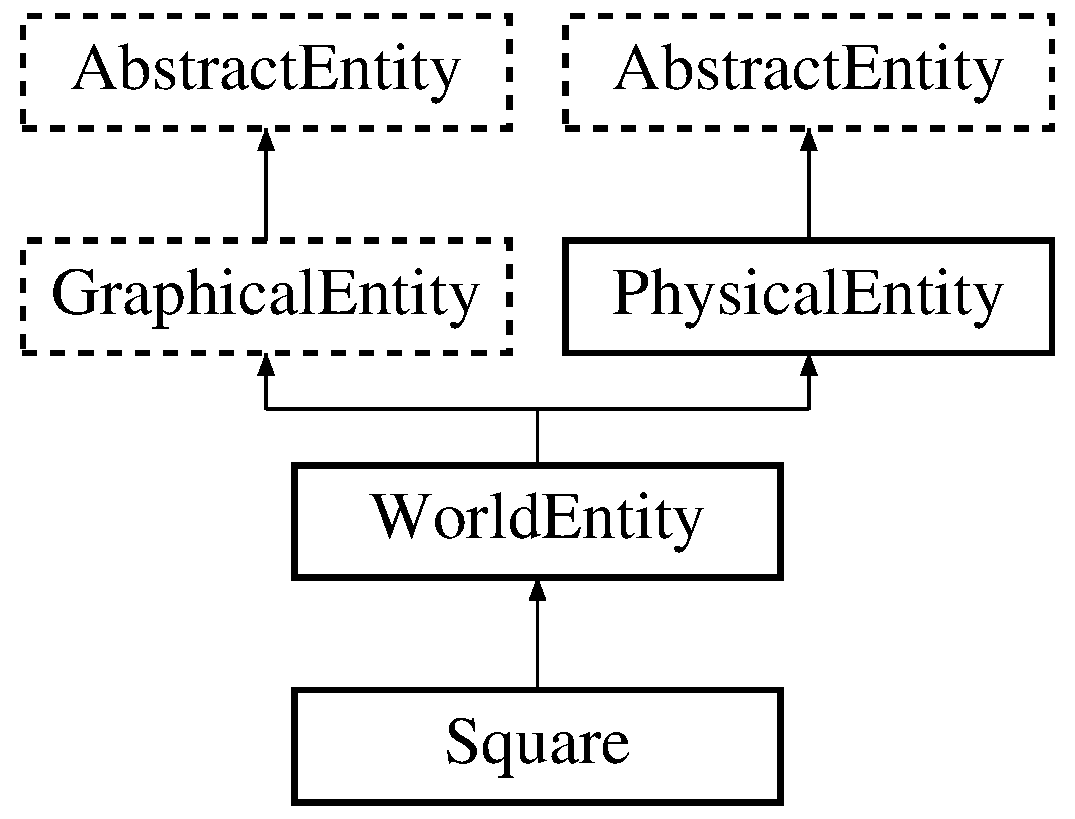
\includegraphics[height=4.000000cm]{class_square}
\end{center}
\end{figure}
\subsection*{Public Member Functions}
\begin{DoxyCompactItemize}
\item 
\hyperlink{class_square_a3c81cb469cb4f7c496617ba020c35582}{Square} (b2\+World const $\ast$\hyperlink{class_physical_entity_ae6c23c3817c4d7f9a867abed05cd7834}{world}, b2\+Body $\ast$\hyperlink{class_physical_entity_a91a5016393dd890c490b329abd938ec7}{body})
\item 
virtual void \hyperlink{class_square_a64094ed22922bb6f98271dbd26be408b}{on\+Begin\+Contact} (b2\+Contact $\ast$contact)
\begin{DoxyCompactList}\small\item\em Contains what the entity should do when a contact begins. \end{DoxyCompactList}\item 
virtual void \hyperlink{class_square_a42f034da822a46094e943f1b617b727e}{on\+End\+Contact} (b2\+Contact $\ast$contact)
\begin{DoxyCompactList}\small\item\em Contains what the entity shoukd do when a contact ends. \end{DoxyCompactList}\item 
virtual void \hyperlink{class_square_afb90e037b269f878406d52bee92e7290}{tick} (void)
\begin{DoxyCompactList}\small\item\em Runs a physical frame of the entity. \end{DoxyCompactList}\item 
void \hyperlink{class_square_ac7b9e76c633bbb107f0af3e48ffa90f8}{impulse\+Down} (void)
\item 
std\+::string \hyperlink{class_square_ae58ee8ae5092447d175966a617bc70ec}{get\+Info} (void) const 
\item 
void \hyperlink{class_square_a0166e843739e678f8a286f525b4b5662}{jump} (void)
\end{DoxyCompactItemize}
\subsection*{Static Public Member Functions}
\begin{DoxyCompactItemize}
\item 
static b2\+Body\+Def \hyperlink{class_square_a69e35e679ca51e9b1c48e41a53c810db}{get\+Body\+Def} (void)
\end{DoxyCompactItemize}
\subsection*{Protected Attributes}
\begin{DoxyCompactItemize}
\item 
bool \hyperlink{class_square_a353e98336921e4244ed66482262e5773}{contact\+Left}
\item 
bool \hyperlink{class_square_ab96608d72e01b3ebffd37bed24b6d070}{contact\+Right}
\item 
bool \hyperlink{class_square_a67729d52489abe1b988e4385100ba5cf}{contact\+Bottom\+Right}
\item 
bool \hyperlink{class_square_aca8a8366a0056f73f520998f4bf1fbbe}{contact\+Bottom\+Left}
\item 
int \hyperlink{class_square_a3c52d1135e840b92f50d5a74f19c7b51}{num\+Foot\+Contacts}
\end{DoxyCompactItemize}
\subsection*{Additional Inherited Members}


\subsection{Constructor \& Destructor Documentation}
\hypertarget{class_square_a3c81cb469cb4f7c496617ba020c35582}{}\index{Square@{Square}!Square@{Square}}
\index{Square@{Square}!Square@{Square}}
\subsubsection[{Square(b2\+World const $\ast$world, b2\+Body $\ast$body)}]{\setlength{\rightskip}{0pt plus 5cm}Square\+::\+Square (
\begin{DoxyParamCaption}
\item[{b2\+World const $\ast$}]{world, }
\item[{b2\+Body $\ast$}]{body}
\end{DoxyParamCaption}
)}\label{class_square_a3c81cb469cb4f7c496617ba020c35582}


\subsection{Member Function Documentation}
\hypertarget{class_square_a69e35e679ca51e9b1c48e41a53c810db}{}\index{Square@{Square}!get\+Body\+Def@{get\+Body\+Def}}
\index{get\+Body\+Def@{get\+Body\+Def}!Square@{Square}}
\subsubsection[{get\+Body\+Def(void)}]{\setlength{\rightskip}{0pt plus 5cm}b2\+Body\+Def Square\+::get\+Body\+Def (
\begin{DoxyParamCaption}
\item[{void}]{}
\end{DoxyParamCaption}
)\hspace{0.3cm}{\ttfamily [static]}}\label{class_square_a69e35e679ca51e9b1c48e41a53c810db}
\hypertarget{class_square_ae58ee8ae5092447d175966a617bc70ec}{}\index{Square@{Square}!get\+Info@{get\+Info}}
\index{get\+Info@{get\+Info}!Square@{Square}}
\subsubsection[{get\+Info(void) const }]{\setlength{\rightskip}{0pt plus 5cm}std\+::string Square\+::get\+Info (
\begin{DoxyParamCaption}
\item[{void}]{}
\end{DoxyParamCaption}
) const}\label{class_square_ae58ee8ae5092447d175966a617bc70ec}
\hypertarget{class_square_ac7b9e76c633bbb107f0af3e48ffa90f8}{}\index{Square@{Square}!impulse\+Down@{impulse\+Down}}
\index{impulse\+Down@{impulse\+Down}!Square@{Square}}
\subsubsection[{impulse\+Down(void)}]{\setlength{\rightskip}{0pt plus 5cm}void Square\+::impulse\+Down (
\begin{DoxyParamCaption}
\item[{void}]{}
\end{DoxyParamCaption}
)}\label{class_square_ac7b9e76c633bbb107f0af3e48ffa90f8}
\hypertarget{class_square_a0166e843739e678f8a286f525b4b5662}{}\index{Square@{Square}!jump@{jump}}
\index{jump@{jump}!Square@{Square}}
\subsubsection[{jump(void)}]{\setlength{\rightskip}{0pt plus 5cm}void Square\+::jump (
\begin{DoxyParamCaption}
\item[{void}]{}
\end{DoxyParamCaption}
)}\label{class_square_a0166e843739e678f8a286f525b4b5662}
\hypertarget{class_square_a64094ed22922bb6f98271dbd26be408b}{}\index{Square@{Square}!on\+Begin\+Contact@{on\+Begin\+Contact}}
\index{on\+Begin\+Contact@{on\+Begin\+Contact}!Square@{Square}}
\subsubsection[{on\+Begin\+Contact(b2\+Contact $\ast$contact)}]{\setlength{\rightskip}{0pt plus 5cm}void Square\+::on\+Begin\+Contact (
\begin{DoxyParamCaption}
\item[{b2\+Contact $\ast$}]{contact}
\end{DoxyParamCaption}
)\hspace{0.3cm}{\ttfamily [virtual]}}\label{class_square_a64094ed22922bb6f98271dbd26be408b}


Contains what the entity should do when a contact begins. 


\begin{DoxyParams}{Parameters}
{\em contact} & The contact information. \\
\hline
\end{DoxyParams}


Reimplemented from \hyperlink{class_physical_entity_a61e9f273e51f5855ca0bf7bb842c738d}{Physical\+Entity}.

\hypertarget{class_square_a42f034da822a46094e943f1b617b727e}{}\index{Square@{Square}!on\+End\+Contact@{on\+End\+Contact}}
\index{on\+End\+Contact@{on\+End\+Contact}!Square@{Square}}
\subsubsection[{on\+End\+Contact(b2\+Contact $\ast$contact)}]{\setlength{\rightskip}{0pt plus 5cm}void Square\+::on\+End\+Contact (
\begin{DoxyParamCaption}
\item[{b2\+Contact $\ast$}]{contact}
\end{DoxyParamCaption}
)\hspace{0.3cm}{\ttfamily [virtual]}}\label{class_square_a42f034da822a46094e943f1b617b727e}


Contains what the entity shoukd do when a contact ends. 


\begin{DoxyParams}{Parameters}
{\em contact} & The contact information. \\
\hline
\end{DoxyParams}


Reimplemented from \hyperlink{class_physical_entity_ae2a98ad512ba0169dcca7bb5b4223306}{Physical\+Entity}.

\hypertarget{class_square_afb90e037b269f878406d52bee92e7290}{}\index{Square@{Square}!tick@{tick}}
\index{tick@{tick}!Square@{Square}}
\subsubsection[{tick(void)}]{\setlength{\rightskip}{0pt plus 5cm}void Square\+::tick (
\begin{DoxyParamCaption}
\item[{void}]{}
\end{DoxyParamCaption}
)\hspace{0.3cm}{\ttfamily [virtual]}}\label{class_square_afb90e037b269f878406d52bee92e7290}


Runs a physical frame of the entity. 



Implements \hyperlink{class_abstract_entity_ac5602c7978aa4eaff46aa206f06046d7}{Abstract\+Entity}.



\subsection{Member Data Documentation}
\hypertarget{class_square_aca8a8366a0056f73f520998f4bf1fbbe}{}\index{Square@{Square}!contact\+Bottom\+Left@{contact\+Bottom\+Left}}
\index{contact\+Bottom\+Left@{contact\+Bottom\+Left}!Square@{Square}}
\subsubsection[{contact\+Bottom\+Left}]{\setlength{\rightskip}{0pt plus 5cm}bool Square\+::contact\+Bottom\+Left\hspace{0.3cm}{\ttfamily [protected]}}\label{class_square_aca8a8366a0056f73f520998f4bf1fbbe}
\hypertarget{class_square_a67729d52489abe1b988e4385100ba5cf}{}\index{Square@{Square}!contact\+Bottom\+Right@{contact\+Bottom\+Right}}
\index{contact\+Bottom\+Right@{contact\+Bottom\+Right}!Square@{Square}}
\subsubsection[{contact\+Bottom\+Right}]{\setlength{\rightskip}{0pt plus 5cm}bool Square\+::contact\+Bottom\+Right\hspace{0.3cm}{\ttfamily [protected]}}\label{class_square_a67729d52489abe1b988e4385100ba5cf}
\hypertarget{class_square_a353e98336921e4244ed66482262e5773}{}\index{Square@{Square}!contact\+Left@{contact\+Left}}
\index{contact\+Left@{contact\+Left}!Square@{Square}}
\subsubsection[{contact\+Left}]{\setlength{\rightskip}{0pt plus 5cm}bool Square\+::contact\+Left\hspace{0.3cm}{\ttfamily [protected]}}\label{class_square_a353e98336921e4244ed66482262e5773}
\hypertarget{class_square_ab96608d72e01b3ebffd37bed24b6d070}{}\index{Square@{Square}!contact\+Right@{contact\+Right}}
\index{contact\+Right@{contact\+Right}!Square@{Square}}
\subsubsection[{contact\+Right}]{\setlength{\rightskip}{0pt plus 5cm}bool Square\+::contact\+Right\hspace{0.3cm}{\ttfamily [protected]}}\label{class_square_ab96608d72e01b3ebffd37bed24b6d070}
\hypertarget{class_square_a3c52d1135e840b92f50d5a74f19c7b51}{}\index{Square@{Square}!num\+Foot\+Contacts@{num\+Foot\+Contacts}}
\index{num\+Foot\+Contacts@{num\+Foot\+Contacts}!Square@{Square}}
\subsubsection[{num\+Foot\+Contacts}]{\setlength{\rightskip}{0pt plus 5cm}int Square\+::num\+Foot\+Contacts\hspace{0.3cm}{\ttfamily [protected]}}\label{class_square_a3c52d1135e840b92f50d5a74f19c7b51}


The documentation for this class was generated from the following files\+:\begin{DoxyCompactItemize}
\item 
Entity/\+Entities/\hyperlink{_square_8hpp}{Square.\+hpp}\item 
Entity/\+Entities/\hyperlink{_square_8cpp}{Square.\+cpp}\end{DoxyCompactItemize}

\hypertarget{class_test_level}{}\section{Test\+Level Class Reference}
\label{class_test_level}\index{Test\+Level@{Test\+Level}}


Contains the \hyperlink{class_test_level}{Test\+Level} class declaration.  




{\ttfamily \#include $<$Test\+Level.\+hpp$>$}

Inheritance diagram for Test\+Level\+:\begin{figure}[H]
\begin{center}
\leavevmode
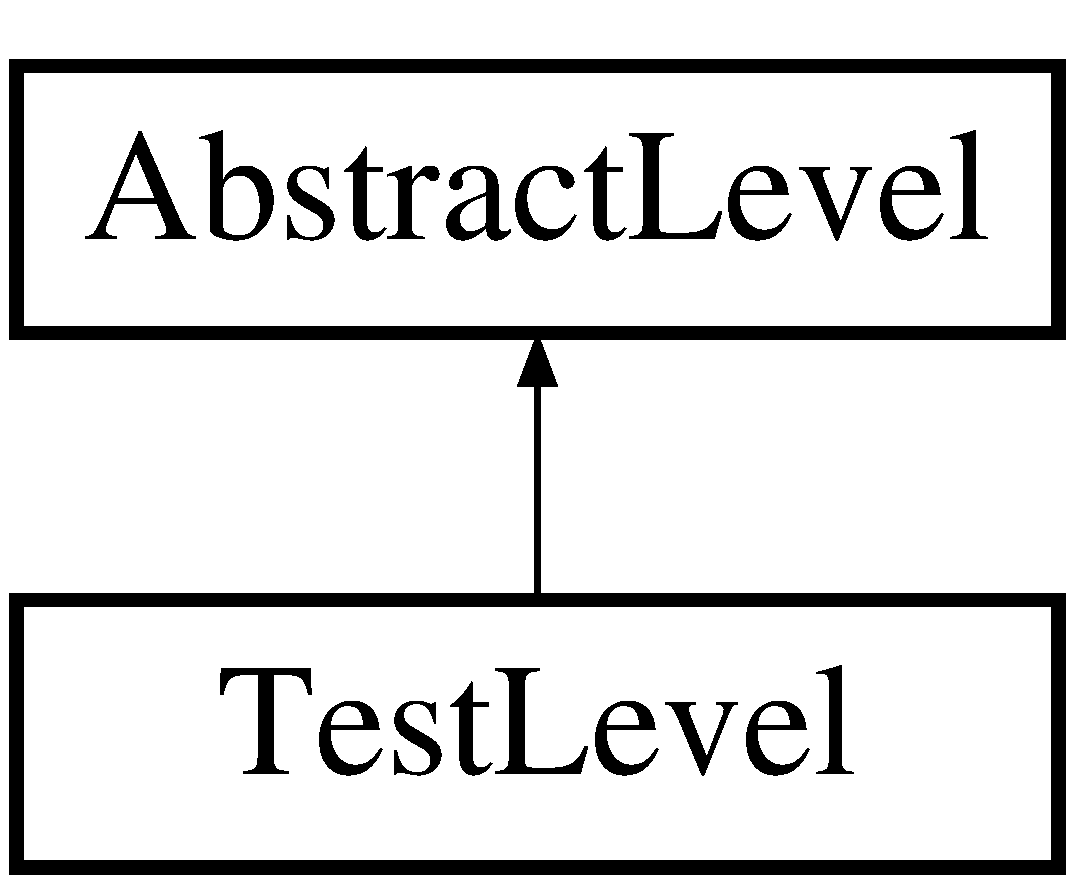
\includegraphics[height=2.000000cm]{class_test_level}
\end{center}
\end{figure}
\subsection*{Public Member Functions}
\begin{DoxyCompactItemize}
\item 
\hyperlink{class_test_level_a5f5e91dab534ad6e17ca716f11c7274a}{Test\+Level} (b2\+World \&\hyperlink{class_abstract_level_a566499434bbd056afd9e12b971e8a41e}{world}, sf\+::\+Render\+Window \&\hyperlink{class_abstract_level_a3332e1be17da924be26064ac4e089721}{window})
\item 
virtual void \hyperlink{class_test_level_a4be8aacf1a305c58b7670de20d6f4303}{initialize} (void)
\begin{DoxyCompactList}\small\item\em Initializes the level. Creates the entities and put them in the entity lists, among other things. \end{DoxyCompactList}\item 
virtual void \hyperlink{class_test_level_a299cc2d19d10678e932bf2df65fe9902}{tick} (void)
\begin{DoxyCompactList}\small\item\em Game tick. Runs a physical frame of the level. \end{DoxyCompactList}\item 
virtual void \hyperlink{class_test_level_a840787cff2a1941a5ce4fafe31433094}{render} (void)
\begin{DoxyCompactList}\small\item\em Render method. Renders the level on screen. \end{DoxyCompactList}\item 
virtual bool \hyperlink{class_test_level_a2644a0797dc2224ff9088a4c87e71b2b}{is\+Finished} (void)
\begin{DoxyCompactList}\small\item\em Tells whether or not the level is finished. \end{DoxyCompactList}\item 
virtual void \hyperlink{class_test_level_a4f16d4600d4b2aeb9299af3417977539}{poll\+Event} (sf\+::\+Event e)
\begin{DoxyCompactList}\small\item\em Handles an event caught by the window. \end{DoxyCompactList}\end{DoxyCompactItemize}
\subsection*{Protected Attributes}
\begin{DoxyCompactItemize}
\item 
\hyperlink{class_square}{Square} $\ast$ \hyperlink{class_test_level_a122398737974e85c0c652cc8b07b74b8}{player}
\item 
sf\+::\+Text \hyperlink{class_test_level_a230d13d6ab7b2b95c971a49e732710ca}{fps\+Text}
\item 
sf\+::\+Text \hyperlink{class_test_level_a55f3d8b00469758c027c4788357fe535}{player\+Info\+Text}
\item 
sf\+::\+Clock \hyperlink{class_test_level_a856b65cd7d74f6f283dc467e9ed954df}{fps\+Clock}
\end{DoxyCompactItemize}


\subsection{Detailed Description}
Contains the \hyperlink{class_test_level}{Test\+Level} class declaration. 

\begin{DoxyAuthor}{Author}
Roch Dionnet
\end{DoxyAuthor}
A level used for testing. 

\subsection{Constructor \& Destructor Documentation}
\hypertarget{class_test_level_a5f5e91dab534ad6e17ca716f11c7274a}{}\index{Test\+Level@{Test\+Level}!Test\+Level@{Test\+Level}}
\index{Test\+Level@{Test\+Level}!Test\+Level@{Test\+Level}}
\subsubsection[{Test\+Level(b2\+World \&world, sf\+::\+Render\+Window \&window)}]{\setlength{\rightskip}{0pt plus 5cm}Test\+Level\+::\+Test\+Level (
\begin{DoxyParamCaption}
\item[{b2\+World \&}]{world, }
\item[{sf\+::\+Render\+Window \&}]{window}
\end{DoxyParamCaption}
)}\label{class_test_level_a5f5e91dab534ad6e17ca716f11c7274a}


\subsection{Member Function Documentation}
\hypertarget{class_test_level_a4be8aacf1a305c58b7670de20d6f4303}{}\index{Test\+Level@{Test\+Level}!initialize@{initialize}}
\index{initialize@{initialize}!Test\+Level@{Test\+Level}}
\subsubsection[{initialize(void)}]{\setlength{\rightskip}{0pt plus 5cm}void Test\+Level\+::initialize (
\begin{DoxyParamCaption}
\item[{void}]{}
\end{DoxyParamCaption}
)\hspace{0.3cm}{\ttfamily [virtual]}}\label{class_test_level_a4be8aacf1a305c58b7670de20d6f4303}


Initializes the level. Creates the entities and put them in the entity lists, among other things. 



Implements \hyperlink{class_abstract_level_aaac7519d2d31d8db995585dec4f5aec0}{Abstract\+Level}.

\hypertarget{class_test_level_a2644a0797dc2224ff9088a4c87e71b2b}{}\index{Test\+Level@{Test\+Level}!is\+Finished@{is\+Finished}}
\index{is\+Finished@{is\+Finished}!Test\+Level@{Test\+Level}}
\subsubsection[{is\+Finished(void)}]{\setlength{\rightskip}{0pt plus 5cm}bool Test\+Level\+::is\+Finished (
\begin{DoxyParamCaption}
\item[{void}]{}
\end{DoxyParamCaption}
)\hspace{0.3cm}{\ttfamily [virtual]}}\label{class_test_level_a2644a0797dc2224ff9088a4c87e71b2b}


Tells whether or not the level is finished. 

\begin{DoxyReturn}{Returns}
true if the level\textquotesingle{}s end condition is met, else returns false. 
\end{DoxyReturn}


Implements \hyperlink{class_abstract_level_a1dbffd34c5ebd93ff833aa6a23047546}{Abstract\+Level}.

\hypertarget{class_test_level_a4f16d4600d4b2aeb9299af3417977539}{}\index{Test\+Level@{Test\+Level}!poll\+Event@{poll\+Event}}
\index{poll\+Event@{poll\+Event}!Test\+Level@{Test\+Level}}
\subsubsection[{poll\+Event(sf\+::\+Event e)}]{\setlength{\rightskip}{0pt plus 5cm}void Test\+Level\+::poll\+Event (
\begin{DoxyParamCaption}
\item[{sf\+::\+Event}]{e}
\end{DoxyParamCaption}
)\hspace{0.3cm}{\ttfamily [virtual]}}\label{class_test_level_a4f16d4600d4b2aeb9299af3417977539}


Handles an event caught by the window. 


\begin{DoxyParams}{Parameters}
{\em e} & The event to handle. \\
\hline
\end{DoxyParams}


Reimplemented from \hyperlink{class_abstract_level_aa6b84b35f24206c43bb7cc0af1f9dfb5}{Abstract\+Level}.

\hypertarget{class_test_level_a840787cff2a1941a5ce4fafe31433094}{}\index{Test\+Level@{Test\+Level}!render@{render}}
\index{render@{render}!Test\+Level@{Test\+Level}}
\subsubsection[{render(void)}]{\setlength{\rightskip}{0pt plus 5cm}void Test\+Level\+::render (
\begin{DoxyParamCaption}
\item[{void}]{}
\end{DoxyParamCaption}
)\hspace{0.3cm}{\ttfamily [virtual]}}\label{class_test_level_a840787cff2a1941a5ce4fafe31433094}


Render method. Renders the level on screen. 



Reimplemented from \hyperlink{class_abstract_level_aa64f9c76abab71339dc07643472f13ee}{Abstract\+Level}.

\hypertarget{class_test_level_a299cc2d19d10678e932bf2df65fe9902}{}\index{Test\+Level@{Test\+Level}!tick@{tick}}
\index{tick@{tick}!Test\+Level@{Test\+Level}}
\subsubsection[{tick(void)}]{\setlength{\rightskip}{0pt plus 5cm}void Test\+Level\+::tick (
\begin{DoxyParamCaption}
\item[{void}]{}
\end{DoxyParamCaption}
)\hspace{0.3cm}{\ttfamily [virtual]}}\label{class_test_level_a299cc2d19d10678e932bf2df65fe9902}


Game tick. Runs a physical frame of the level. 



Implements \hyperlink{class_abstract_level_ac50b3069600e90000f2f62dccb522154}{Abstract\+Level}.



\subsection{Member Data Documentation}
\hypertarget{class_test_level_a856b65cd7d74f6f283dc467e9ed954df}{}\index{Test\+Level@{Test\+Level}!fps\+Clock@{fps\+Clock}}
\index{fps\+Clock@{fps\+Clock}!Test\+Level@{Test\+Level}}
\subsubsection[{fps\+Clock}]{\setlength{\rightskip}{0pt plus 5cm}sf\+::\+Clock Test\+Level\+::fps\+Clock\hspace{0.3cm}{\ttfamily [protected]}}\label{class_test_level_a856b65cd7d74f6f283dc467e9ed954df}
A clock which is reset each frame, used to count the number of F\+P\+S. \hypertarget{class_test_level_a230d13d6ab7b2b95c971a49e732710ca}{}\index{Test\+Level@{Test\+Level}!fps\+Text@{fps\+Text}}
\index{fps\+Text@{fps\+Text}!Test\+Level@{Test\+Level}}
\subsubsection[{fps\+Text}]{\setlength{\rightskip}{0pt plus 5cm}sf\+::\+Text Test\+Level\+::fps\+Text\hspace{0.3cm}{\ttfamily [protected]}}\label{class_test_level_a230d13d6ab7b2b95c971a49e732710ca}
A text which shows the number of F\+P\+S. \hypertarget{class_test_level_a122398737974e85c0c652cc8b07b74b8}{}\index{Test\+Level@{Test\+Level}!player@{player}}
\index{player@{player}!Test\+Level@{Test\+Level}}
\subsubsection[{player}]{\setlength{\rightskip}{0pt plus 5cm}{\bf Square}$\ast$ Test\+Level\+::player\hspace{0.3cm}{\ttfamily [protected]}}\label{class_test_level_a122398737974e85c0c652cc8b07b74b8}
The rectangle-\/shaped player. \hypertarget{class_test_level_a55f3d8b00469758c027c4788357fe535}{}\index{Test\+Level@{Test\+Level}!player\+Info\+Text@{player\+Info\+Text}}
\index{player\+Info\+Text@{player\+Info\+Text}!Test\+Level@{Test\+Level}}
\subsubsection[{player\+Info\+Text}]{\setlength{\rightskip}{0pt plus 5cm}sf\+::\+Text Test\+Level\+::player\+Info\+Text\hspace{0.3cm}{\ttfamily [protected]}}\label{class_test_level_a55f3d8b00469758c027c4788357fe535}
A text which shows some info on the player. 

The documentation for this class was generated from the following files\+:\begin{DoxyCompactItemize}
\item 
Level/\+Levels/\hyperlink{_test_level_8hpp}{Test\+Level.\+hpp}\item 
Level/\+Levels/\hyperlink{_test_level_8cpp}{Test\+Level.\+cpp}\end{DoxyCompactItemize}

\hypertarget{class_trail_bullet}{}\section{Trail\+Bullet Class Reference}
\label{class_trail_bullet}\index{Trail\+Bullet@{Trail\+Bullet}}


{\ttfamily \#include $<$Trail\+Bullet.\+hpp$>$}

Inheritance diagram for Trail\+Bullet\+:\begin{figure}[H]
\begin{center}
\leavevmode
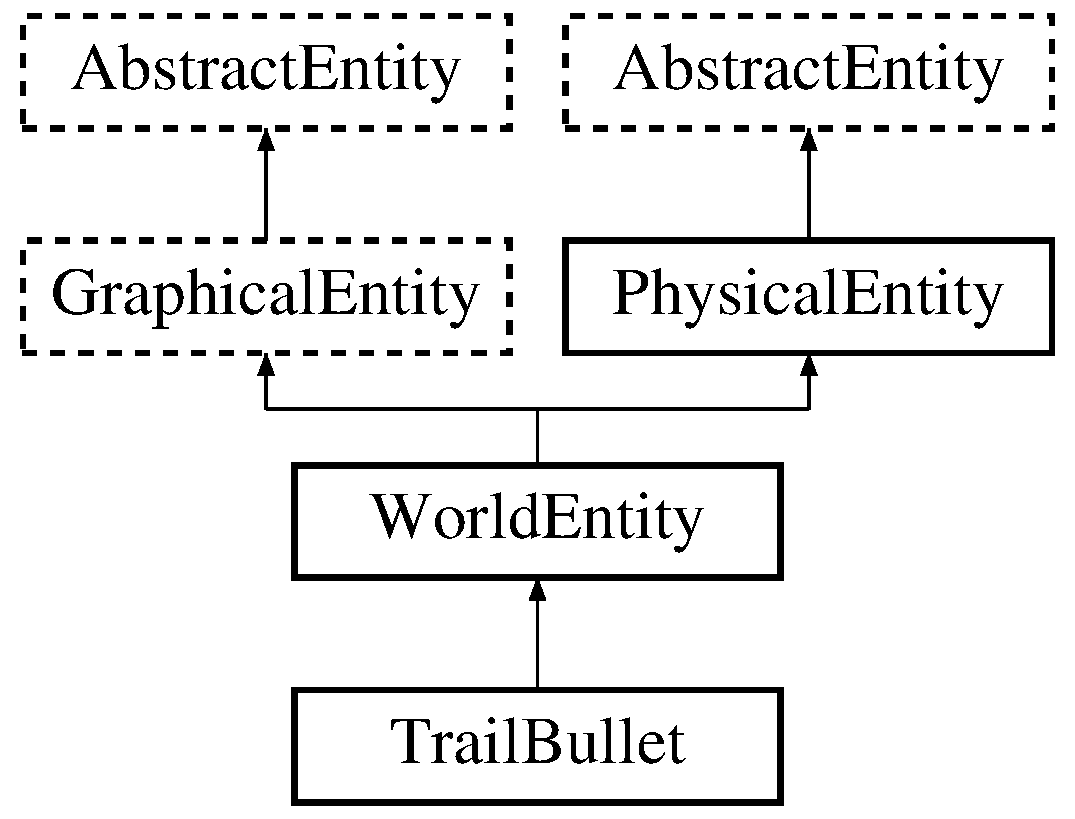
\includegraphics[height=4.000000cm]{class_trail_bullet}
\end{center}
\end{figure}
\subsection*{Public Member Functions}
\begin{DoxyCompactItemize}
\item 
\hyperlink{class_trail_bullet_a4eb109da5dd108d1174a7c1ddb7ca9e1}{Trail\+Bullet} (b2\+World const $\ast$\hyperlink{class_physical_entity_ae6c23c3817c4d7f9a867abed05cd7834}{world}, b2\+Body $\ast$\hyperlink{class_physical_entity_a91a5016393dd890c490b329abd938ec7}{body}, b2\+Vec2 pos, bool \hyperlink{class_trail_bullet_a20902ecccf91729dcc6e3e00fba5b420}{direction\+Is\+Right})
\item 
virtual void \hyperlink{class_trail_bullet_a3fe11738249bc471194e2eb207730911}{tick} (void)
\begin{DoxyCompactList}\small\item\em Runs a physical frame of the entity. \end{DoxyCompactList}\item 
virtual void \hyperlink{class_trail_bullet_adc085681d9e19e335c5ec083fc291a5f}{on\+Begin\+Contact} (b2\+Contact $\ast$contact)
\begin{DoxyCompactList}\small\item\em Contains what the entity should do when a contact begins. \end{DoxyCompactList}\end{DoxyCompactItemize}
\subsection*{Static Public Member Functions}
\begin{DoxyCompactItemize}
\item 
static b2\+Body\+Def \hyperlink{class_trail_bullet_a418bfa9338a78fbe3c8aff5a46cbdbd1}{get\+Body\+Def} (void)
\end{DoxyCompactItemize}
\subsection*{Protected Attributes}
\begin{DoxyCompactItemize}
\item 
bool \hyperlink{class_trail_bullet_a20902ecccf91729dcc6e3e00fba5b420}{direction\+Is\+Right}
\item 
float \hyperlink{class_trail_bullet_a5c2df82f2d6910c7366db8d12e3fa8ac}{start\+X}
\end{DoxyCompactItemize}
\subsection*{Additional Inherited Members}


\subsection{Constructor \& Destructor Documentation}
\hypertarget{class_trail_bullet_a4eb109da5dd108d1174a7c1ddb7ca9e1}{}\index{Trail\+Bullet@{Trail\+Bullet}!Trail\+Bullet@{Trail\+Bullet}}
\index{Trail\+Bullet@{Trail\+Bullet}!Trail\+Bullet@{Trail\+Bullet}}
\subsubsection[{Trail\+Bullet(b2\+World const $\ast$world, b2\+Body $\ast$body, b2\+Vec2 pos, bool direction\+Is\+Right)}]{\setlength{\rightskip}{0pt plus 5cm}Trail\+Bullet\+::\+Trail\+Bullet (
\begin{DoxyParamCaption}
\item[{b2\+World const $\ast$}]{world, }
\item[{b2\+Body $\ast$}]{body, }
\item[{b2\+Vec2}]{pos, }
\item[{bool}]{direction\+Is\+Right}
\end{DoxyParamCaption}
)}\label{class_trail_bullet_a4eb109da5dd108d1174a7c1ddb7ca9e1}


\subsection{Member Function Documentation}
\hypertarget{class_trail_bullet_a418bfa9338a78fbe3c8aff5a46cbdbd1}{}\index{Trail\+Bullet@{Trail\+Bullet}!get\+Body\+Def@{get\+Body\+Def}}
\index{get\+Body\+Def@{get\+Body\+Def}!Trail\+Bullet@{Trail\+Bullet}}
\subsubsection[{get\+Body\+Def(void)}]{\setlength{\rightskip}{0pt plus 5cm}b2\+Body\+Def Trail\+Bullet\+::get\+Body\+Def (
\begin{DoxyParamCaption}
\item[{void}]{}
\end{DoxyParamCaption}
)\hspace{0.3cm}{\ttfamily [static]}}\label{class_trail_bullet_a418bfa9338a78fbe3c8aff5a46cbdbd1}
\hypertarget{class_trail_bullet_adc085681d9e19e335c5ec083fc291a5f}{}\index{Trail\+Bullet@{Trail\+Bullet}!on\+Begin\+Contact@{on\+Begin\+Contact}}
\index{on\+Begin\+Contact@{on\+Begin\+Contact}!Trail\+Bullet@{Trail\+Bullet}}
\subsubsection[{on\+Begin\+Contact(b2\+Contact $\ast$contact)}]{\setlength{\rightskip}{0pt plus 5cm}void Trail\+Bullet\+::on\+Begin\+Contact (
\begin{DoxyParamCaption}
\item[{b2\+Contact $\ast$}]{contact}
\end{DoxyParamCaption}
)\hspace{0.3cm}{\ttfamily [virtual]}}\label{class_trail_bullet_adc085681d9e19e335c5ec083fc291a5f}


Contains what the entity should do when a contact begins. 


\begin{DoxyParams}{Parameters}
{\em contact} & The contact information. \\
\hline
\end{DoxyParams}


Reimplemented from \hyperlink{class_physical_entity_a61e9f273e51f5855ca0bf7bb842c738d}{Physical\+Entity}.

\hypertarget{class_trail_bullet_a3fe11738249bc471194e2eb207730911}{}\index{Trail\+Bullet@{Trail\+Bullet}!tick@{tick}}
\index{tick@{tick}!Trail\+Bullet@{Trail\+Bullet}}
\subsubsection[{tick(void)}]{\setlength{\rightskip}{0pt plus 5cm}void Trail\+Bullet\+::tick (
\begin{DoxyParamCaption}
\item[{void}]{}
\end{DoxyParamCaption}
)\hspace{0.3cm}{\ttfamily [virtual]}}\label{class_trail_bullet_a3fe11738249bc471194e2eb207730911}


Runs a physical frame of the entity. 



Implements \hyperlink{class_abstract_entity_ac5602c7978aa4eaff46aa206f06046d7}{Abstract\+Entity}.



\subsection{Member Data Documentation}
\hypertarget{class_trail_bullet_a20902ecccf91729dcc6e3e00fba5b420}{}\index{Trail\+Bullet@{Trail\+Bullet}!direction\+Is\+Right@{direction\+Is\+Right}}
\index{direction\+Is\+Right@{direction\+Is\+Right}!Trail\+Bullet@{Trail\+Bullet}}
\subsubsection[{direction\+Is\+Right}]{\setlength{\rightskip}{0pt plus 5cm}bool Trail\+Bullet\+::direction\+Is\+Right\hspace{0.3cm}{\ttfamily [protected]}}\label{class_trail_bullet_a20902ecccf91729dcc6e3e00fba5b420}
\hypertarget{class_trail_bullet_a5c2df82f2d6910c7366db8d12e3fa8ac}{}\index{Trail\+Bullet@{Trail\+Bullet}!start\+X@{start\+X}}
\index{start\+X@{start\+X}!Trail\+Bullet@{Trail\+Bullet}}
\subsubsection[{start\+X}]{\setlength{\rightskip}{0pt plus 5cm}float Trail\+Bullet\+::start\+X\hspace{0.3cm}{\ttfamily [protected]}}\label{class_trail_bullet_a5c2df82f2d6910c7366db8d12e3fa8ac}


The documentation for this class was generated from the following files\+:\begin{DoxyCompactItemize}
\item 
Entity/\+Entities/\hyperlink{_trail_bullet_8hpp}{Trail\+Bullet.\+hpp}\item 
Entity/\+Entities/\hyperlink{_trail_bullet_8cpp}{Trail\+Bullet.\+cpp}\end{DoxyCompactItemize}

\hypertarget{class_world_entity}{}\section{World\+Entity Class Reference}
\label{class_world_entity}\index{World\+Entity@{World\+Entity}}


Contains the \hyperlink{class_world_entity}{World\+Entity} class declaration.  




{\ttfamily \#include $<$World\+Entity.\+hpp$>$}

Inheritance diagram for World\+Entity\+:\begin{figure}[H]
\begin{center}
\leavevmode
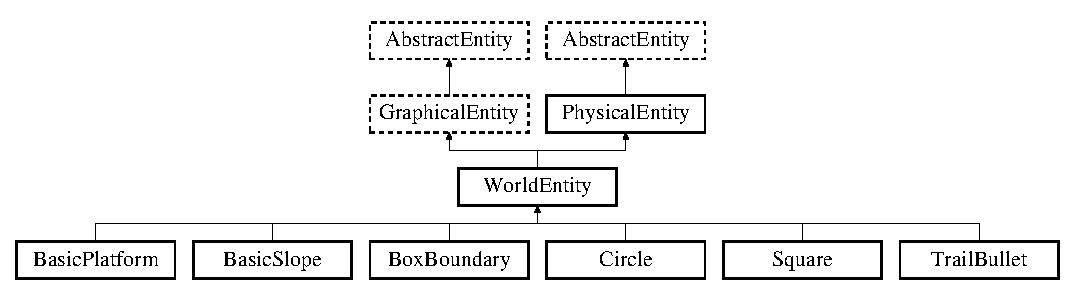
\includegraphics[height=3.522013cm]{class_world_entity}
\end{center}
\end{figure}
\subsection*{Public Member Functions}
\begin{DoxyCompactItemize}
\item 
\hyperlink{class_world_entity_ad41912aa528f517bbed6c0e60f4f8c52}{World\+Entity} (b2\+World const $\ast$\hyperlink{class_physical_entity_ae6c23c3817c4d7f9a867abed05cd7834}{world}, b2\+Body $\ast$\hyperlink{class_physical_entity_a91a5016393dd890c490b329abd938ec7}{body})
\begin{DoxyCompactList}\small\item\em Constructor. \end{DoxyCompactList}\end{DoxyCompactItemize}
\subsection*{Protected Member Functions}
\begin{DoxyCompactItemize}
\item 
void \hyperlink{class_world_entity_a526ecc62c6bf6703a197cd35840125ef}{update\+Graphics} (void)
\begin{DoxyCompactList}\small\item\em Update the graphics to match the physics in terms of transform. \end{DoxyCompactList}\end{DoxyCompactItemize}
\subsection*{Additional Inherited Members}


\subsection{Detailed Description}
Contains the \hyperlink{class_world_entity}{World\+Entity} class declaration. 

\begin{DoxyAuthor}{Author}
Roch Dionnet
\end{DoxyAuthor}
represents a game element that has both a physical and a graphical existence. 

\subsection{Constructor \& Destructor Documentation}
\hypertarget{class_world_entity_ad41912aa528f517bbed6c0e60f4f8c52}{}\index{World\+Entity@{World\+Entity}!World\+Entity@{World\+Entity}}
\index{World\+Entity@{World\+Entity}!World\+Entity@{World\+Entity}}
\subsubsection[{World\+Entity(b2\+World const $\ast$world, b2\+Body $\ast$body)}]{\setlength{\rightskip}{0pt plus 5cm}World\+Entity\+::\+World\+Entity (
\begin{DoxyParamCaption}
\item[{b2\+World const $\ast$}]{world, }
\item[{b2\+Body $\ast$}]{body}
\end{DoxyParamCaption}
)\hspace{0.3cm}{\ttfamily [inline]}}\label{class_world_entity_ad41912aa528f517bbed6c0e60f4f8c52}


Constructor. 


\begin{DoxyParams}{Parameters}
{\em world} & \\
\hline
{\em body} & \\
\hline
\end{DoxyParams}
\begin{DoxySeeAlso}{See also}
\hyperlink{class_physical_entity_ae6c23c3817c4d7f9a867abed05cd7834}{Physical\+Entity\+::world}, \hyperlink{class_physical_entity_a91a5016393dd890c490b329abd938ec7}{Physical\+Entity\+::body} 
\end{DoxySeeAlso}


\subsection{Member Function Documentation}
\hypertarget{class_world_entity_a526ecc62c6bf6703a197cd35840125ef}{}\index{World\+Entity@{World\+Entity}!update\+Graphics@{update\+Graphics}}
\index{update\+Graphics@{update\+Graphics}!World\+Entity@{World\+Entity}}
\subsubsection[{update\+Graphics(void)}]{\setlength{\rightskip}{0pt plus 5cm}void World\+Entity\+::update\+Graphics (
\begin{DoxyParamCaption}
\item[{void}]{}
\end{DoxyParamCaption}
)\hspace{0.3cm}{\ttfamily [protected]}}\label{class_world_entity_a526ecc62c6bf6703a197cd35840125ef}


Update the graphics to match the physics in terms of transform. 



The documentation for this class was generated from the following files\+:\begin{DoxyCompactItemize}
\item 
Entity/\hyperlink{_world_entity_8hpp}{World\+Entity.\+hpp}\item 
Entity/\hyperlink{_world_entity_8cpp}{World\+Entity.\+cpp}\end{DoxyCompactItemize}

\chapter{File Documentation}
\hypertarget{constants_8hpp}{}\section{constants.\+hpp File Reference}
\label{constants_8hpp}\index{constants.\+hpp@{constants.\+hpp}}
\subsection*{Macros}
\begin{DoxyCompactItemize}
\item 
\#define \hyperlink{constants_8hpp_a322d53d23d7208a9e6a86b52db9732d1}{P\+P\+M}~32.f
\begin{DoxyCompactList}\small\item\em Defines some global constants, such as the pixels per meter conversion value. \end{DoxyCompactList}\item 
\#define \hyperlink{constants_8hpp_ac55f9c1a8887709eacdde68f0d745c48}{C\+L\+E\+A\+R\+C\+O\+L\+O\+R}~sf\+::\+Color\+::\+White
\end{DoxyCompactItemize}


\subsection{Macro Definition Documentation}
\hypertarget{constants_8hpp_ac55f9c1a8887709eacdde68f0d745c48}{}\index{constants.\+hpp@{constants.\+hpp}!C\+L\+E\+A\+R\+C\+O\+L\+O\+R@{C\+L\+E\+A\+R\+C\+O\+L\+O\+R}}
\index{C\+L\+E\+A\+R\+C\+O\+L\+O\+R@{C\+L\+E\+A\+R\+C\+O\+L\+O\+R}!constants.\+hpp@{constants.\+hpp}}
\subsubsection[{C\+L\+E\+A\+R\+C\+O\+L\+O\+R}]{\setlength{\rightskip}{0pt plus 5cm}\#define C\+L\+E\+A\+R\+C\+O\+L\+O\+R~sf\+::\+Color\+::\+White}\label{constants_8hpp_ac55f9c1a8887709eacdde68f0d745c48}
The clear color used before each frame. \hypertarget{constants_8hpp_a322d53d23d7208a9e6a86b52db9732d1}{}\index{constants.\+hpp@{constants.\+hpp}!P\+P\+M@{P\+P\+M}}
\index{P\+P\+M@{P\+P\+M}!constants.\+hpp@{constants.\+hpp}}
\subsubsection[{P\+P\+M}]{\setlength{\rightskip}{0pt plus 5cm}\#define P\+P\+M~32.f}\label{constants_8hpp_a322d53d23d7208a9e6a86b52db9732d1}


Defines some global constants, such as the pixels per meter conversion value. 

\begin{DoxyAuthor}{Author}
Roch Dionnet\+The pixels per meter conversion value. 
\end{DoxyAuthor}

\hypertarget{_abstract_entity_8hpp}{}\section{Entity/\+Abstract\+Entity.hpp File Reference}
\label{_abstract_entity_8hpp}\index{Entity/\+Abstract\+Entity.\+hpp@{Entity/\+Abstract\+Entity.\+hpp}}
\subsection*{Classes}
\begin{DoxyCompactItemize}
\item 
class \hyperlink{class_abstract_entity}{Abstract\+Entity}
\begin{DoxyCompactList}\small\item\em Contains the \hyperlink{class_abstract_entity}{Abstract\+Entity} class declaration. \end{DoxyCompactList}\end{DoxyCompactItemize}

\hypertarget{_basic_platform_8cpp}{}\section{Entity/\+Entities/\+Basic\+Platform.cpp File Reference}
\label{_basic_platform_8cpp}\index{Entity/\+Entities/\+Basic\+Platform.\+cpp@{Entity/\+Entities/\+Basic\+Platform.\+cpp}}
{\ttfamily \#include \char`\"{}Basic\+Platform.\+hpp\char`\"{}}\\*
{\ttfamily \#include \char`\"{}../../constants.\+hpp\char`\"{}}\\*
{\ttfamily \#include \char`\"{}../../sfml\+To\+Box2\+D.\+hpp\char`\"{}}\\*

\hypertarget{_basic_platform_8hpp}{}\section{Entity/\+Entities/\+Basic\+Platform.hpp File Reference}
\label{_basic_platform_8hpp}\index{Entity/\+Entities/\+Basic\+Platform.\+hpp@{Entity/\+Entities/\+Basic\+Platform.\+hpp}}
{\ttfamily \#include \char`\"{}../\+World\+Entity.\+hpp\char`\"{}}\\*
{\ttfamily \#include $<$iostream$>$}\\*
{\ttfamily \#include \char`\"{}../../sfml\+To\+Box2\+D.\+hpp\char`\"{}}\\*
\subsection*{Classes}
\begin{DoxyCompactItemize}
\item 
class \hyperlink{class_basic_platform}{Basic\+Platform}
\end{DoxyCompactItemize}

\hypertarget{_basic_slope_8cpp}{}\section{Entity/\+Entities/\+Basic\+Slope.cpp File Reference}
\label{_basic_slope_8cpp}\index{Entity/\+Entities/\+Basic\+Slope.\+cpp@{Entity/\+Entities/\+Basic\+Slope.\+cpp}}
{\ttfamily \#include \char`\"{}Basic\+Slope.\+hpp\char`\"{}}\\*
{\ttfamily \#include \char`\"{}../../constants.\+hpp\char`\"{}}\\*

\hypertarget{_basic_slope_8hpp}{}\section{Entity/\+Entities/\+Basic\+Slope.hpp File Reference}
\label{_basic_slope_8hpp}\index{Entity/\+Entities/\+Basic\+Slope.\+hpp@{Entity/\+Entities/\+Basic\+Slope.\+hpp}}
{\ttfamily \#include \char`\"{}../\+World\+Entity.\+hpp\char`\"{}}\\*
\subsection*{Classes}
\begin{DoxyCompactItemize}
\item 
class \hyperlink{class_basic_slope}{Basic\+Slope}
\end{DoxyCompactItemize}

\hypertarget{_box_boundary_8cpp}{}\section{Entity/\+Entities/\+Box\+Boundary.cpp File Reference}
\label{_box_boundary_8cpp}\index{Entity/\+Entities/\+Box\+Boundary.\+cpp@{Entity/\+Entities/\+Box\+Boundary.\+cpp}}
{\ttfamily \#include \char`\"{}Box\+Boundary.\+hpp\char`\"{}}\\*
{\ttfamily \#include $<$cmath$>$}\\*

\hypertarget{_box_boundary_8hpp}{}\section{Entity/\+Entities/\+Box\+Boundary.hpp File Reference}
\label{_box_boundary_8hpp}\index{Entity/\+Entities/\+Box\+Boundary.\+hpp@{Entity/\+Entities/\+Box\+Boundary.\+hpp}}
{\ttfamily \#include \char`\"{}../\+World\+Entity.\+hpp\char`\"{}}\\*
{\ttfamily \#include \char`\"{}../../constants.\+hpp\char`\"{}}\\*
\subsection*{Classes}
\begin{DoxyCompactItemize}
\item 
class \hyperlink{class_box_boundary}{Box\+Boundary}
\end{DoxyCompactItemize}

\hypertarget{_circle_8cpp}{}\section{Entity/\+Entities/\+Circle.cpp File Reference}
\label{_circle_8cpp}\index{Entity/\+Entities/\+Circle.\+cpp@{Entity/\+Entities/\+Circle.\+cpp}}
{\ttfamily \#include \char`\"{}Circle.\+hpp\char`\"{}}\\*
{\ttfamily \#include \char`\"{}../../constants.\+hpp\char`\"{}}\\*

\hypertarget{_circle_8hpp}{}\section{Entity/\+Entities/\+Circle.hpp File Reference}
\label{_circle_8hpp}\index{Entity/\+Entities/\+Circle.\+hpp@{Entity/\+Entities/\+Circle.\+hpp}}
{\ttfamily \#include \char`\"{}../\+World\+Entity.\+hpp\char`\"{}}\\*
\subsection*{Classes}
\begin{DoxyCompactItemize}
\item 
class \hyperlink{class_circle}{Circle}
\end{DoxyCompactItemize}

\hypertarget{_square_8cpp}{}\section{Entity/\+Entities/\+Square.cpp File Reference}
\label{_square_8cpp}\index{Entity/\+Entities/\+Square.\+cpp@{Entity/\+Entities/\+Square.\+cpp}}
{\ttfamily \#include \char`\"{}Square.\+hpp\char`\"{}}\\*
{\ttfamily \#include $<$iostream$>$}\\*
{\ttfamily \#include \char`\"{}../../constants.\+hpp\char`\"{}}\\*

\hypertarget{_square_8hpp}{}\section{Entity/\+Entities/\+Square.hpp File Reference}
\label{_square_8hpp}\index{Entity/\+Entities/\+Square.\+hpp@{Entity/\+Entities/\+Square.\+hpp}}
{\ttfamily \#include \char`\"{}../\+World\+Entity.\+hpp\char`\"{}}\\*
\subsection*{Classes}
\begin{DoxyCompactItemize}
\item 
class \hyperlink{class_square}{Square}
\end{DoxyCompactItemize}

\hypertarget{_trail_bullet_8cpp}{}\section{Entity/\+Entities/\+Trail\+Bullet.cpp File Reference}
\label{_trail_bullet_8cpp}\index{Entity/\+Entities/\+Trail\+Bullet.\+cpp@{Entity/\+Entities/\+Trail\+Bullet.\+cpp}}
{\ttfamily \#include \char`\"{}Trail\+Bullet.\+hpp\char`\"{}}\\*
{\ttfamily \#include \char`\"{}../../constants.\+hpp\char`\"{}}\\*

\hypertarget{_trail_bullet_8hpp}{}\section{Entity/\+Entities/\+Trail\+Bullet.hpp File Reference}
\label{_trail_bullet_8hpp}\index{Entity/\+Entities/\+Trail\+Bullet.\+hpp@{Entity/\+Entities/\+Trail\+Bullet.\+hpp}}
{\ttfamily \#include \char`\"{}../\+World\+Entity.\+hpp\char`\"{}}\\*
\subsection*{Classes}
\begin{DoxyCompactItemize}
\item 
class \hyperlink{class_trail_bullet}{Trail\+Bullet}
\end{DoxyCompactItemize}

\hypertarget{_entity_contact_listener_8cpp}{}\section{Entity/\+Entity\+Contact\+Listener.cpp File Reference}
\label{_entity_contact_listener_8cpp}\index{Entity/\+Entity\+Contact\+Listener.\+cpp@{Entity/\+Entity\+Contact\+Listener.\+cpp}}
{\ttfamily \#include \char`\"{}Entity\+Contact\+Listener.\+hpp\char`\"{}}\\*
{\ttfamily \#include \char`\"{}Entities/\+Square.\+hpp\char`\"{}}\\*

\hypertarget{_entity_contact_listener_8hpp}{}\section{Entity/\+Entity\+Contact\+Listener.hpp File Reference}
\label{_entity_contact_listener_8hpp}\index{Entity/\+Entity\+Contact\+Listener.\+hpp@{Entity/\+Entity\+Contact\+Listener.\+hpp}}
{\ttfamily \#include $<$Box2\+D/\+Box2\+D.\+h$>$}\\*
\subsection*{Classes}
\begin{DoxyCompactItemize}
\item 
class \hyperlink{class_entity_contact_listener}{Entity\+Contact\+Listener}
\begin{DoxyCompactList}\small\item\em Contains the \hyperlink{class_entity_contact_listener}{Entity\+Contact\+Listener} class declaration. \end{DoxyCompactList}\end{DoxyCompactItemize}

\hypertarget{_graphical_entity_8hpp}{}\section{Entity/\+Graphical\+Entity.hpp File Reference}
\label{_graphical_entity_8hpp}\index{Entity/\+Graphical\+Entity.\+hpp@{Entity/\+Graphical\+Entity.\+hpp}}
{\ttfamily \#include \char`\"{}Abstract\+Entity.\+hpp\char`\"{}}\\*
{\ttfamily \#include $<$S\+F\+M\+L/\+Graphics.\+hpp$>$}\\*
\subsection*{Classes}
\begin{DoxyCompactItemize}
\item 
class \hyperlink{class_graphical_element}{Graphical\+Element}
\begin{DoxyCompactList}\small\item\em Contains the \hyperlink{class_graphical_entity}{Graphical\+Entity} and \hyperlink{class_graphical_element}{Graphical\+Element} class declarations. \end{DoxyCompactList}\item 
class \hyperlink{class_graphical_entity}{Graphical\+Entity}
\begin{DoxyCompactList}\small\item\em Represents a game element that can be displayed. \end{DoxyCompactList}\end{DoxyCompactItemize}

\hypertarget{_physical_entity_8hpp}{}\section{Entity/\+Physical\+Entity.hpp File Reference}
\label{_physical_entity_8hpp}\index{Entity/\+Physical\+Entity.\+hpp@{Entity/\+Physical\+Entity.\+hpp}}
{\ttfamily \#include $<$Box2\+D/\+Box2\+D.\+h$>$}\\*
{\ttfamily \#include \char`\"{}Abstract\+Entity.\+hpp\char`\"{}}\\*
\subsection*{Classes}
\begin{DoxyCompactItemize}
\item 
class \hyperlink{class_physical_entity}{Physical\+Entity}
\begin{DoxyCompactList}\small\item\em Contains the \hyperlink{class_physical_entity}{Physical\+Entity} class declaration. \end{DoxyCompactList}\end{DoxyCompactItemize}

\hypertarget{_world_entity_8cpp}{}\section{Entity/\+World\+Entity.cpp File Reference}
\label{_world_entity_8cpp}\index{Entity/\+World\+Entity.\+cpp@{Entity/\+World\+Entity.\+cpp}}
{\ttfamily \#include \char`\"{}World\+Entity.\+hpp\char`\"{}}\\*
{\ttfamily \#include \char`\"{}../constants.\+hpp\char`\"{}}\\*

\hypertarget{_world_entity_8hpp}{}\section{Entity/\+World\+Entity.hpp File Reference}
\label{_world_entity_8hpp}\index{Entity/\+World\+Entity.\+hpp@{Entity/\+World\+Entity.\+hpp}}
{\ttfamily \#include \char`\"{}Physical\+Entity.\+hpp\char`\"{}}\\*
{\ttfamily \#include \char`\"{}Graphical\+Entity.\+hpp\char`\"{}}\\*
{\ttfamily \#include \char`\"{}../constants.\+hpp\char`\"{}}\\*
\subsection*{Classes}
\begin{DoxyCompactItemize}
\item 
class \hyperlink{class_world_entity}{World\+Entity}
\begin{DoxyCompactList}\small\item\em Contains the \hyperlink{class_world_entity}{World\+Entity} class declaration. \end{DoxyCompactList}\end{DoxyCompactItemize}

\hypertarget{_abstract_level_8cpp}{}\section{Level/\+Abstract\+Level.cpp File Reference}
\label{_abstract_level_8cpp}\index{Level/\+Abstract\+Level.\+cpp@{Level/\+Abstract\+Level.\+cpp}}
{\ttfamily \#include \char`\"{}Abstract\+Level.\+hpp\char`\"{}}\\*

\hypertarget{_abstract_level_8hpp}{}\section{Level/\+Abstract\+Level.hpp File Reference}
\label{_abstract_level_8hpp}\index{Level/\+Abstract\+Level.\+hpp@{Level/\+Abstract\+Level.\+hpp}}
{\ttfamily \#include $<$Box2\+D/\+Box2\+D.\+h$>$}\\*
{\ttfamily \#include $<$S\+F\+M\+L/\+Graphics.\+hpp$>$}\\*
{\ttfamily \#include \char`\"{}../\+Entity/\+Graphical\+Entity.\+hpp\char`\"{}}\\*
{\ttfamily \#include \char`\"{}../\+Entity/\+Physical\+Entity.\+hpp\char`\"{}}\\*
\subsection*{Classes}
\begin{DoxyCompactItemize}
\item 
class \hyperlink{class_abstract_level}{Abstract\+Level}
\begin{DoxyCompactList}\small\item\em Represents a basic linear level, with an end condition. \end{DoxyCompactList}\end{DoxyCompactItemize}
\subsection*{Typedefs}
\begin{DoxyCompactItemize}
\item 
typedef std\+::vector$<$ \hyperlink{class_graphical_entity}{Graphical\+Entity} $\ast$ $>$ \hyperlink{_abstract_level_8hpp_a33f40c5b921668406bc9359321c92e00}{Graphical\+Entity\+List}
\begin{DoxyCompactList}\small\item\em Contains the \hyperlink{class_abstract_level}{Abstract\+Level} class declaration. \end{DoxyCompactList}\item 
typedef std\+::vector$<$ \hyperlink{class_physical_entity}{Physical\+Entity} $\ast$ $>$ \hyperlink{_abstract_level_8hpp_a2f8ec60783d4f4d3911b30a32c604d3e}{Physical\+Entity\+List}
\end{DoxyCompactItemize}


\subsection{Typedef Documentation}
\hypertarget{_abstract_level_8hpp_a33f40c5b921668406bc9359321c92e00}{}\index{Abstract\+Level.\+hpp@{Abstract\+Level.\+hpp}!Graphical\+Entity\+List@{Graphical\+Entity\+List}}
\index{Graphical\+Entity\+List@{Graphical\+Entity\+List}!Abstract\+Level.\+hpp@{Abstract\+Level.\+hpp}}
\subsubsection[{Graphical\+Entity\+List}]{\setlength{\rightskip}{0pt plus 5cm}typedef std\+::vector$<${\bf Graphical\+Entity}$\ast$$>$ {\bf Graphical\+Entity\+List}}\label{_abstract_level_8hpp_a33f40c5b921668406bc9359321c92e00}


Contains the \hyperlink{class_abstract_level}{Abstract\+Level} class declaration. 

\begin{DoxyAuthor}{Author}
Roch Dionnet 
\end{DoxyAuthor}
\hypertarget{_abstract_level_8hpp_a2f8ec60783d4f4d3911b30a32c604d3e}{}\index{Abstract\+Level.\+hpp@{Abstract\+Level.\+hpp}!Physical\+Entity\+List@{Physical\+Entity\+List}}
\index{Physical\+Entity\+List@{Physical\+Entity\+List}!Abstract\+Level.\+hpp@{Abstract\+Level.\+hpp}}
\subsubsection[{Physical\+Entity\+List}]{\setlength{\rightskip}{0pt plus 5cm}typedef std\+::vector$<${\bf Physical\+Entity}$\ast$$>$ {\bf Physical\+Entity\+List}}\label{_abstract_level_8hpp_a2f8ec60783d4f4d3911b30a32c604d3e}

\hypertarget{_test_level_8cpp}{}\section{Level/\+Levels/\+Test\+Level.cpp File Reference}
\label{_test_level_8cpp}\index{Level/\+Levels/\+Test\+Level.\+cpp@{Level/\+Levels/\+Test\+Level.\+cpp}}
{\ttfamily \#include $<$iostream$>$}\\*
{\ttfamily \#include $<$sstream$>$}\\*
{\ttfamily \#include \char`\"{}Test\+Level.\+hpp\char`\"{}}\\*
{\ttfamily \#include \char`\"{}../../\+Entity/\+Entities/\+Basic\+Platform.\+hpp\char`\"{}}\\*
{\ttfamily \#include \char`\"{}../../\+Entity/\+Entities/\+Basic\+Slope.\+hpp\char`\"{}}\\*
{\ttfamily \#include \char`\"{}../../\+Entity/\+Entities/\+Square.\+hpp\char`\"{}}\\*
{\ttfamily \#include \char`\"{}../../\+Entity/\+Entities/\+Box\+Boundary.\+hpp\char`\"{}}\\*
{\ttfamily \#include \char`\"{}../../constants.\+hpp\char`\"{}}\\*
{\ttfamily \#include \char`\"{}../../sfml\+To\+Box2\+D.\+hpp\char`\"{}}\\*
{\ttfamily \#include \char`\"{}../../\+Entity/\+Entity\+Contact\+Listener.\+hpp\char`\"{}}\\*

\hypertarget{_test_level_8hpp}{}\section{Level/\+Levels/\+Test\+Level.hpp File Reference}
\label{_test_level_8hpp}\index{Level/\+Levels/\+Test\+Level.\+hpp@{Level/\+Levels/\+Test\+Level.\+hpp}}
{\ttfamily \#include \char`\"{}../\+Abstract\+Level.\+hpp\char`\"{}}\\*
{\ttfamily \#include \char`\"{}../../\+Entity/\+Entities/\+Square.\+hpp\char`\"{}}\\*
\subsection*{Classes}
\begin{DoxyCompactItemize}
\item 
class \hyperlink{class_test_level}{Test\+Level}
\begin{DoxyCompactList}\small\item\em Contains the \hyperlink{class_test_level}{Test\+Level} class declaration. \end{DoxyCompactList}\end{DoxyCompactItemize}

\hypertarget{main_8cpp}{}\section{main.\+cpp File Reference}
\label{main_8cpp}\index{main.\+cpp@{main.\+cpp}}
{\ttfamily \#include $<$iostream$>$}\\*
{\ttfamily \#include $<$Box2\+D/\+Box2\+D.\+h$>$}\\*
{\ttfamily \#include $<$S\+F\+M\+L/\+Graphics.\+hpp$>$}\\*
{\ttfamily \#include $<$sstream$>$}\\*
{\ttfamily \#include $<$iterator$>$}\\*
{\ttfamily \#include $<$cmath$>$}\\*
{\ttfamily \#include \char`\"{}Entity/\+World\+Entity.\+hpp\char`\"{}}\\*
{\ttfamily \#include \char`\"{}Entity/\+Entity\+Contact\+Listener.\+hpp\char`\"{}}\\*
{\ttfamily \#include \char`\"{}Entity/\+Entities/\+Square.\+hpp\char`\"{}}\\*
{\ttfamily \#include \char`\"{}Entity/\+Entities/\+Basic\+Platform.\+hpp\char`\"{}}\\*
{\ttfamily \#include \char`\"{}Entity/\+Entities/\+Box\+Boundary.\+hpp\char`\"{}}\\*
{\ttfamily \#include \char`\"{}Entity/\+Entities/\+Trail\+Bullet.\+hpp\char`\"{}}\\*
{\ttfamily \#include \char`\"{}constants.\+hpp\char`\"{}}\\*
{\ttfamily \#include \char`\"{}sfml\+To\+Box2\+D.\+hpp\char`\"{}}\\*
{\ttfamily \#include \char`\"{}Level/\+Abstract\+Level.\+hpp\char`\"{}}\\*
{\ttfamily \#include \char`\"{}Level/\+Levels/\+Test\+Level.\+hpp\char`\"{}}\\*
\subsection*{Typedefs}
\begin{DoxyCompactItemize}
\item 
typedef std\+::vector$<$ \hyperlink{class_physical_entity}{Physical\+Entity} $\ast$ $>$ \hyperlink{main_8cpp_a2f8ec60783d4f4d3911b30a32c604d3e}{Physical\+Entity\+List}
\item 
typedef std\+::vector$<$ \hyperlink{class_graphical_entity}{Graphical\+Entity} $\ast$ $>$ \hyperlink{main_8cpp_a33f40c5b921668406bc9359321c92e00}{Graphical\+Entity\+List}
\end{DoxyCompactItemize}
\subsection*{Functions}
\begin{DoxyCompactItemize}
\item 
{\footnotesize template$<$typename T\+Num $>$ }\\std\+::string \hyperlink{main_8cpp_a76bcff87353bed53d79858061c3e127f}{num\+To\+Str} (T\+Num num)
\begin{DoxyCompactList}\small\item\em main file \end{DoxyCompactList}\item 
int \hyperlink{main_8cpp_ae66f6b31b5ad750f1fe042a706a4e3d4}{main} ()
\begin{DoxyCompactList}\small\item\em Main function. \end{DoxyCompactList}\end{DoxyCompactItemize}


\subsection{Typedef Documentation}
\hypertarget{main_8cpp_a33f40c5b921668406bc9359321c92e00}{}\index{main.\+cpp@{main.\+cpp}!Graphical\+Entity\+List@{Graphical\+Entity\+List}}
\index{Graphical\+Entity\+List@{Graphical\+Entity\+List}!main.\+cpp@{main.\+cpp}}
\subsubsection[{Graphical\+Entity\+List}]{\setlength{\rightskip}{0pt plus 5cm}typedef std\+::vector$<${\bf Graphical\+Entity}$\ast$$>$ {\bf Graphical\+Entity\+List}}\label{main_8cpp_a33f40c5b921668406bc9359321c92e00}
\hypertarget{main_8cpp_a2f8ec60783d4f4d3911b30a32c604d3e}{}\index{main.\+cpp@{main.\+cpp}!Physical\+Entity\+List@{Physical\+Entity\+List}}
\index{Physical\+Entity\+List@{Physical\+Entity\+List}!main.\+cpp@{main.\+cpp}}
\subsubsection[{Physical\+Entity\+List}]{\setlength{\rightskip}{0pt plus 5cm}typedef std\+::vector$<${\bf Physical\+Entity}$\ast$$>$ {\bf Physical\+Entity\+List}}\label{main_8cpp_a2f8ec60783d4f4d3911b30a32c604d3e}


\subsection{Function Documentation}
\hypertarget{main_8cpp_ae66f6b31b5ad750f1fe042a706a4e3d4}{}\index{main.\+cpp@{main.\+cpp}!main@{main}}
\index{main@{main}!main.\+cpp@{main.\+cpp}}
\subsubsection[{main()}]{\setlength{\rightskip}{0pt plus 5cm}int main (
\begin{DoxyParamCaption}
{}
\end{DoxyParamCaption}
)}\label{main_8cpp_ae66f6b31b5ad750f1fe042a706a4e3d4}


Main function. 

\begin{DoxyReturn}{Returns}
E\+X\+I\+T\+\_\+\+S\+U\+C\+C\+E\+S\+S -\/ The program exited successfully.
\end{DoxyReturn}
Entry point of the program. Contains the game loop, instanciates levels... \hypertarget{main_8cpp_a76bcff87353bed53d79858061c3e127f}{}\index{main.\+cpp@{main.\+cpp}!num\+To\+Str@{num\+To\+Str}}
\index{num\+To\+Str@{num\+To\+Str}!main.\+cpp@{main.\+cpp}}
\subsubsection[{num\+To\+Str(\+T\+Num num)}]{\setlength{\rightskip}{0pt plus 5cm}template$<$typename T\+Num $>$ std\+::string num\+To\+Str (
\begin{DoxyParamCaption}
\item[{T\+Num}]{num}
\end{DoxyParamCaption}
)}\label{main_8cpp_a76bcff87353bed53d79858061c3e127f}


main file 

\begin{DoxyAuthor}{Author}
Roch Dionnet
\end{DoxyAuthor}
Converts a numerical value (int, float...) into an std\+::string. 
\begin{DoxyParams}{Parameters}
{\em num} & The numerical value. \\
\hline
\end{DoxyParams}
\begin{DoxyReturn}{Returns}
The numerical value converted into an std\+::string. 
\end{DoxyReturn}

\hypertarget{sfml_to_box2_d_8cpp}{}\section{sfml\+To\+Box2\+D.\+cpp File Reference}
\label{sfml_to_box2_d_8cpp}\index{sfml\+To\+Box2\+D.\+cpp@{sfml\+To\+Box2\+D.\+cpp}}
{\ttfamily \#include \char`\"{}sfml\+To\+Box2\+D.\+hpp\char`\"{}}\\*
{\ttfamily \#include \char`\"{}constants.\+hpp\char`\"{}}\\*
\subsection*{Functions}
\begin{DoxyCompactItemize}
\item 
sf\+::\+Vector2f \hyperlink{sfml_to_box2_d_8cpp_a8a4dbaaf617e7765ec939695e66a36b2}{physical\+Vec\+To\+Graphical\+Vec} (b2\+Vec2 const \&b2vec)
\begin{DoxyCompactList}\small\item\em Provides some function that convert Box2\+D units into S\+F\+M\+L units and vice-\/versa. \end{DoxyCompactList}\item 
b2\+Vec2 \hyperlink{sfml_to_box2_d_8cpp_ae4470ad6d4f3e86df57412ae3dd3dbbc}{graphical\+Vec\+To\+Physical\+Vec} (sf\+::\+Vector2f const \&sfvec)
\begin{DoxyCompactList}\small\item\em Converts an S\+F\+M\+L Vector2f vector into a Box2\+D b2\+Vec2 vector. \end{DoxyCompactList}\end{DoxyCompactItemize}


\subsection{Function Documentation}
\hypertarget{sfml_to_box2_d_8cpp_ae4470ad6d4f3e86df57412ae3dd3dbbc}{}\index{sfml\+To\+Box2\+D.\+cpp@{sfml\+To\+Box2\+D.\+cpp}!graphical\+Vec\+To\+Physical\+Vec@{graphical\+Vec\+To\+Physical\+Vec}}
\index{graphical\+Vec\+To\+Physical\+Vec@{graphical\+Vec\+To\+Physical\+Vec}!sfml\+To\+Box2\+D.\+cpp@{sfml\+To\+Box2\+D.\+cpp}}
\subsubsection[{graphical\+Vec\+To\+Physical\+Vec(sf\+::\+Vector2f const \&sfvec)}]{\setlength{\rightskip}{0pt plus 5cm}b2\+Vec2 graphical\+Vec\+To\+Physical\+Vec (
\begin{DoxyParamCaption}
\item[{sf\+::\+Vector2f const \&}]{sfvec}
\end{DoxyParamCaption}
)}\label{sfml_to_box2_d_8cpp_ae4470ad6d4f3e86df57412ae3dd3dbbc}


Converts an S\+F\+M\+L Vector2f vector into a Box2\+D b2\+Vec2 vector. 


\begin{DoxyParams}{Parameters}
{\em sfvec} & The Vector2f vector to be converted. \\
\hline
\end{DoxyParams}
\begin{DoxyReturn}{Returns}
The converted b2\+Vec2 vector. 
\end{DoxyReturn}
\hypertarget{sfml_to_box2_d_8cpp_a8a4dbaaf617e7765ec939695e66a36b2}{}\index{sfml\+To\+Box2\+D.\+cpp@{sfml\+To\+Box2\+D.\+cpp}!physical\+Vec\+To\+Graphical\+Vec@{physical\+Vec\+To\+Graphical\+Vec}}
\index{physical\+Vec\+To\+Graphical\+Vec@{physical\+Vec\+To\+Graphical\+Vec}!sfml\+To\+Box2\+D.\+cpp@{sfml\+To\+Box2\+D.\+cpp}}
\subsubsection[{physical\+Vec\+To\+Graphical\+Vec(b2\+Vec2 const \&b2vec)}]{\setlength{\rightskip}{0pt plus 5cm}sf\+::\+Vector2f physical\+Vec\+To\+Graphical\+Vec (
\begin{DoxyParamCaption}
\item[{b2\+Vec2 const \&}]{b2vec}
\end{DoxyParamCaption}
)}\label{sfml_to_box2_d_8cpp_a8a4dbaaf617e7765ec939695e66a36b2}


Provides some function that convert Box2\+D units into S\+F\+M\+L units and vice-\/versa. 

\begin{DoxyAuthor}{Author}
Roch Dionnet
\end{DoxyAuthor}
Converts an S\+F\+M\+L Vector2f vector into a Box2\+D b2\+Vec2 vector. 
\begin{DoxyParams}{Parameters}
{\em b2vec} & The Vector2f vector to be converted. \\
\hline
\end{DoxyParams}
\begin{DoxyReturn}{Returns}
The converted b2\+Vec2 vector. 
\end{DoxyReturn}

\hypertarget{sfml_to_box2_d_8hpp}{}\section{sfml\+To\+Box2\+D.\+hpp File Reference}
\label{sfml_to_box2_d_8hpp}\index{sfml\+To\+Box2\+D.\+hpp@{sfml\+To\+Box2\+D.\+hpp}}
{\ttfamily \#include $<$S\+F\+M\+L/\+Graphics.\+hpp$>$}\\*
{\ttfamily \#include $<$Box2\+D/\+Box2\+D.\+h$>$}\\*
\subsection*{Functions}
\begin{DoxyCompactItemize}
\item 
sf\+::\+Vector2f \hyperlink{sfml_to_box2_d_8hpp_a8a4dbaaf617e7765ec939695e66a36b2}{physical\+Vec\+To\+Graphical\+Vec} (b2\+Vec2 const \&b2vec)
\begin{DoxyCompactList}\small\item\em Provides some function that convert Box2\+D units into S\+F\+M\+L units and vice-\/versa. \end{DoxyCompactList}\item 
b2\+Vec2 \hyperlink{sfml_to_box2_d_8hpp_ae4470ad6d4f3e86df57412ae3dd3dbbc}{graphical\+Vec\+To\+Physical\+Vec} (sf\+::\+Vector2f const \&sfvec)
\begin{DoxyCompactList}\small\item\em Converts an S\+F\+M\+L Vector2f vector into a Box2\+D b2\+Vec2 vector. \end{DoxyCompactList}\end{DoxyCompactItemize}


\subsection{Function Documentation}
\hypertarget{sfml_to_box2_d_8hpp_ae4470ad6d4f3e86df57412ae3dd3dbbc}{}\index{sfml\+To\+Box2\+D.\+hpp@{sfml\+To\+Box2\+D.\+hpp}!graphical\+Vec\+To\+Physical\+Vec@{graphical\+Vec\+To\+Physical\+Vec}}
\index{graphical\+Vec\+To\+Physical\+Vec@{graphical\+Vec\+To\+Physical\+Vec}!sfml\+To\+Box2\+D.\+hpp@{sfml\+To\+Box2\+D.\+hpp}}
\subsubsection[{graphical\+Vec\+To\+Physical\+Vec(sf\+::\+Vector2f const \&sfvec)}]{\setlength{\rightskip}{0pt plus 5cm}b2\+Vec2 graphical\+Vec\+To\+Physical\+Vec (
\begin{DoxyParamCaption}
\item[{sf\+::\+Vector2f const \&}]{sfvec}
\end{DoxyParamCaption}
)}\label{sfml_to_box2_d_8hpp_ae4470ad6d4f3e86df57412ae3dd3dbbc}


Converts an S\+F\+M\+L Vector2f vector into a Box2\+D b2\+Vec2 vector. 


\begin{DoxyParams}{Parameters}
{\em sfvec} & The Vector2f vector to be converted. \\
\hline
\end{DoxyParams}
\begin{DoxyReturn}{Returns}
The converted b2\+Vec2 vector. 
\end{DoxyReturn}
\hypertarget{sfml_to_box2_d_8hpp_a8a4dbaaf617e7765ec939695e66a36b2}{}\index{sfml\+To\+Box2\+D.\+hpp@{sfml\+To\+Box2\+D.\+hpp}!physical\+Vec\+To\+Graphical\+Vec@{physical\+Vec\+To\+Graphical\+Vec}}
\index{physical\+Vec\+To\+Graphical\+Vec@{physical\+Vec\+To\+Graphical\+Vec}!sfml\+To\+Box2\+D.\+hpp@{sfml\+To\+Box2\+D.\+hpp}}
\subsubsection[{physical\+Vec\+To\+Graphical\+Vec(b2\+Vec2 const \&b2vec)}]{\setlength{\rightskip}{0pt plus 5cm}sf\+::\+Vector2f physical\+Vec\+To\+Graphical\+Vec (
\begin{DoxyParamCaption}
\item[{b2\+Vec2 const \&}]{b2vec}
\end{DoxyParamCaption}
)}\label{sfml_to_box2_d_8hpp_a8a4dbaaf617e7765ec939695e66a36b2}


Provides some function that convert Box2\+D units into S\+F\+M\+L units and vice-\/versa. 

\begin{DoxyAuthor}{Author}
Roch Dionnet
\end{DoxyAuthor}
Converts an S\+F\+M\+L Vector2f vector into a Box2\+D b2\+Vec2 vector. 
\begin{DoxyParams}{Parameters}
{\em b2vec} & The Vector2f vector to be converted. \\
\hline
\end{DoxyParams}
\begin{DoxyReturn}{Returns}
The converted b2\+Vec2 vector. 
\end{DoxyReturn}

%--- End generated contents ---

% Index
\backmatter
\newpage
\phantomsection
\clearemptydoublepage
\addcontentsline{toc}{chapter}{Index}
\printindex

\end{document}
